\documentclass[12pt]{article}
\usepackage[latin1]{inputenc}
\usepackage[T1]{fontenc}
\usepackage{palatino}
\usepackage{fancyhdr}
\usepackage{float}
\usepackage{subfigure}
\usepackage{wrapfig}
\usepackage[dvips]{graphics}
\usepackage{graphicx}
\usepackage{epsfig}
\usepackage{multicol}
\usepackage{url}
\usepackage{html}
\usepackage{color}

 \definecolor{violet}{rgb}{0.5,0,0.5}
 
\setlength{\topmargin}{0cm}
\setlength{\headheight}{1cm}
\setlength{\textheight}{21cm}
\setlength{\textwidth}{16cm}
\setlength{\oddsidemargin}{0cm}
\setlength{\evensidemargin}{0cm}
\setlength{\columnsep}{0.125in}
\setlength{\columnseprule}{0.5pt}
\setlength{\footskip}{1cm}
\sloppy

%--------------------------------- page style --------------------------------
\pagestyle{fancy}
\rhead{}
\lhead{}
\rfoot{\thepage}
\lfoot{}
\cfoot{}
%---------------------------------- document ---------------------------------
\date   {}
\title  {Stratus User's Manual}
\author {Sophie Belloeil}

\begin{document}

\setlength{\footrulewidth}{0.6pt}
\maketitle

%%\begin{htmlonly}
%%  \htmlrule
%%  \noindent La version imprimable de ce document est disponible ici~: \\
%%  \begin{center}
%%    \hyperref[hyper]{http://asim.lip6.fr/~jpc/M1-C++/TME/6/TME6.pdf}{}{}
%%                    {http://asim.lip6.fr/~jpc/M1-C++/TME/6/TME6.pdf}
%%  \end{center}
%%\end{htmlonly}

\tableofchildlinks
\htmlrule

\section{What's new}
    \subsection{march 2012}

\begin{itemize}
   \item{A configuration file can be used to direct Stratus.}
   \item{A Stratus's description can now be exported either in Alliance VST format or standard VHDL using the \verb-Save- method and the configuration file.}
   \item{A \verb-Stimuli- method permits to generate stimuli for simulation.}
   \item{Thanks to the \verb-Stimuli- method, a testbench can now automatically be generated either in Alliance PAT format or standard VHDL.}
   \item{The \verb-Simul- method of the class \verb-Model- permits to simulate either with the Alliance's simulator \verb-asimut- or a standard VHDL simulator (\verb-ghdl-).}
\begin{end}



\section{Introduction}
\label{secintroduction}
    
    \subsection{Stratus}
    \label{secstratus}
    \subsubsection{Name}

Stratus -- Procedural design language based upon \emph{Python}

\subsubsection{Description}

\emph{Stratus} is a set of \emph{Python} methods/functions dedicated to procedural generation purposes. From a user point of view, \emph{Stratus} is a circuit's description  language that allows \emph{Python} programming flow control, variable use, and specialized functions in order to handle vlsi objects.\\

\indent Based upon the \emph{Hurricane} data structures, the \emph{Stratus} language gives the user the ability to describe netlist and layout views.

\subsubsection{Creation of a cell}

A cell is a hierachical structural description of a circuit in terms of ports (I/Os), signals (nets) and instances.\\
     
\indent The creation of a cell is done by creating a new class, derivating for class \verb-Model-, with different methods :

\begin{itemize}
\item Method \verb-Interface- : Description of the external ports of the cell :
    \begin{itemize}
        \item SignalIn, SignalOut, ...
    \end{itemize}
\item Method \verb-Netlist- : Description of the netlist of the cell :
    \begin{itemize}
        \item Inst, Signal
    \end{itemize}
\item Method \verb-Layout- : Description of the layout of the cell :
    \begin{itemize}
        \item Place, PlaceTop, PlaceBottom, PlaceRight, PlaceLeft ...
    \end{itemize}
\end{itemize}

\indent Two methods are provided :
\begin{itemize}
    \item Method \verb-View- : Opens/Refreshes the editor in order to see the created layout
    \item Method \verb-Save- : Saves the created cell
    \begin{itemize}
        \item no argument : creation of a netlist file (format file thanks to CRL\_OUT\_LO)
        \item PHYSICAL : creation of a netlist file AND a layout file (format files thanks to CRL\_OUT\_LO and CRL\_OUT\_PH)
        \item STRATUS : creation of a python/stratus file
        \begin{itemize}
            \item FileName : optionnal argument when using Save(STRATUS) in order to choose the name of the file to be generated
            \item Be careful : if one wants to create a stratus file AND a netlist, always use Save(STRATUS) before Save() !
        \end{itemize}
    \end{itemize}
\end{itemize}

\subsubsection{Syntax}

A \emph{Stratus} file must have a .py extension and must begin as follow :
\begin{verbatim}
#!/usr/bin/env python

from stratus import *
\end{verbatim}

\indent The creation of a class is done as follow :
\begin{verbatim}
class myClass ( Model ) :
    ...
    
exemple = myClass ( name, param )
\end{verbatim}

\indent In order to execute a \emph{Stratus} file (named \verb-file- for example), one has two choices :
\begin{verbatim}
python file.py
\end{verbatim}
\indent Or :
\begin{verbatim}
chmod u+x file.py
./file.py
\end{verbatim}

\indent The names used in \emph{Stratus}, as arguments to \emph{Stratus} functions, should be alphanumerical, including the underscore. The arguments of \emph{Stratus} are case sensitive, so \textsc{VDD} is not equivalent to \textsc{vdd}.\\
    
\indent Vectorized connectors or signal can be used using the \textsc{[n:m]} construct.\\

\subsubsection{Syntax highlighting}

When using vi, it's possible to have the right syntax highlighting when using vi :

\begin{itemize}
    \item Commands to do when you want to change once the coloration of your file :
\end{itemize}
\begin{small}
\begin{verbatim}
:syntax off
:source /asim/coriolis/share/etc/stratus.vim
\end{verbatim}
\end{small}
\begin{itemize}
    \item Modification of your .vimrc in order to have the syntax highlighting each time you open a file :
\end{itemize}
\begin{small}
\begin{verbatim}
syntax off
autocmd BufRead,BufNewfile *.py so /asim/coriolis/share/etc/stratus.vim
syntax on
\end{verbatim}
\end{small}
        
\subsubsection{Environment variables}

\begin{itemize}
    \item CRL\_IN\_LO, default value : \verb-def-
    \item CRL\_OUT\_LO, default value : \verb-def-
    \item CRL\_IN\_PH, default value : \verb-def-
    \item CRL\_OUT\_PH, default value : \verb-def-
    \item CRL\_CATA\_LIB, default value : \verb-.-
    \item CRL\_CATAL\_NAME, default value : \verb-CATAL-
\end{itemize}

\begin{htmlonly}

\subsubsection{Example}

You can see a concrete example at : \hyperref[ref]{\emph{Example}}{}{Example}{secexample}

\subsubsection{See Also}

\hyperref[ref]{\emph{Netlist}}{}{Netlist}{secnetlist}
\hyperref[ref]{\emph{Layout}}{}{Layout}{seclayout}
\hyperref[ref]{\emph{Place and Route}}{}{Place and Route}{secroute}
\hyperref[ref]{\emph{Virtual libraty}}{}{Virtual library}{seclibrary}
\hyperref[ref]{\emph{Instanciation facilities}}{}{Instanciation facilities}{secfacilities}

\end{htmlonly}

    \subsection{Example}
    \label{secexample}
    \subsubsection{The addaccu circuit}

\begin{figure}[h!]
\centering
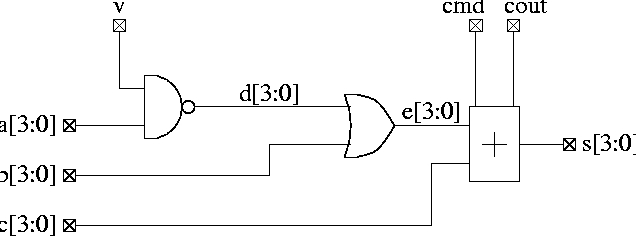
\includegraphics[width=.9\textwidth]{./images/add1.png}
\end{figure}
  
\newpage
\subsubsection{The data-path}

\begin{figure}[h!]
\centering
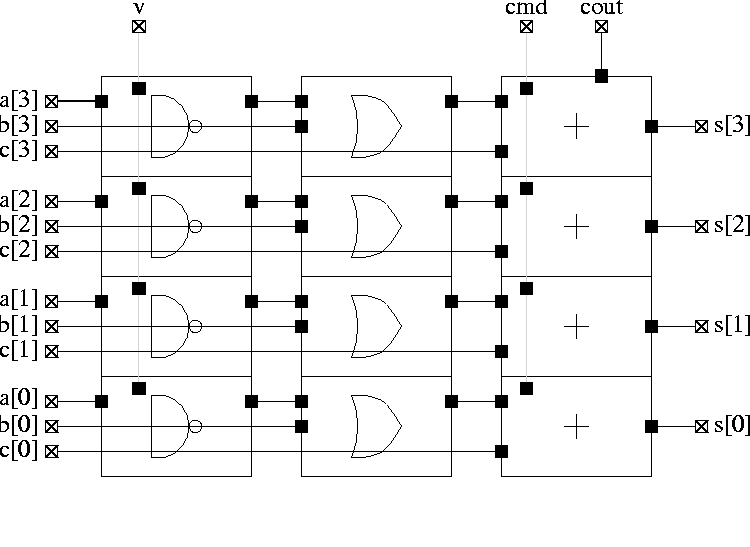
\includegraphics[width=.9\textwidth]{./images/add2.png}
\end{figure}

\newpage
\subsubsection{Description of the circuit with \emph{Stratus} : file addaccu.py}

\begin{figure}[h!]
\centering
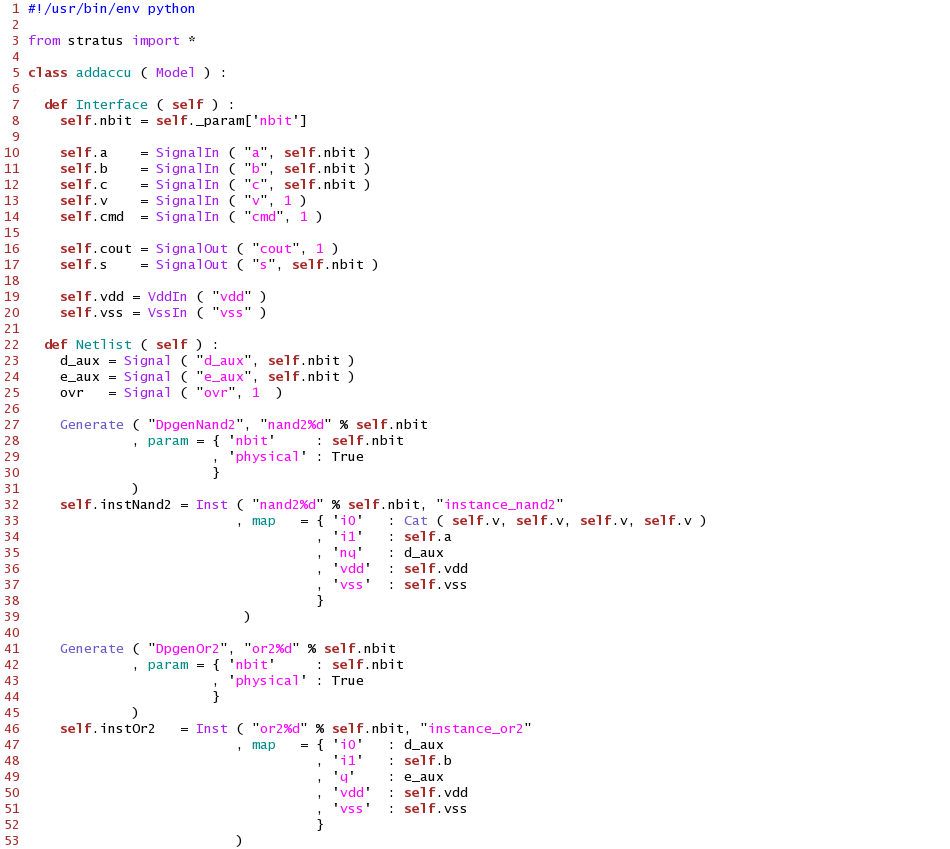
\includegraphics[width=1.4\textwidth]{./images/addaccu1.png}
\end{figure}

\begin{figure}[h!]
\centering
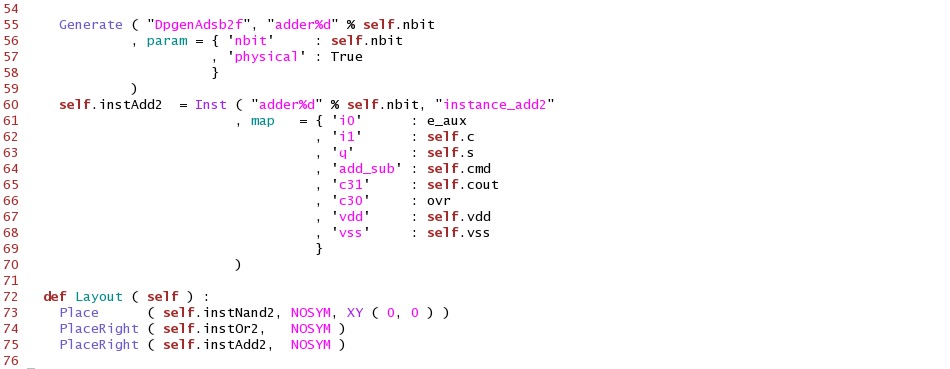
\includegraphics[width=1.4\textwidth]{./images/addaccu2.png}
\end{figure}

\newpage
\subsubsection{Creation of the circuit : file test.py}

\begin{figure}[h!]
\centering
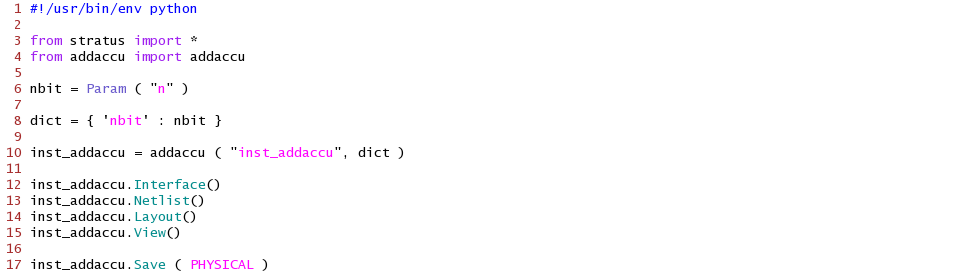
\includegraphics[width=1.4\textwidth]{./images/test.png}
\end{figure}

\subsubsection{How to execute the file}

\begin{verbatim}
python test.py -n 4
\end{verbatim}
\indent or :
\begin{verbatim}
chmod u+x test.py
./test -n 4
\end{verbatim}

\subsubsection{The editor}

The method \verb-View- permits to open an editor in which one can see the cell being created as shown in the picture below.
\begin{figure}[h!]
\centering
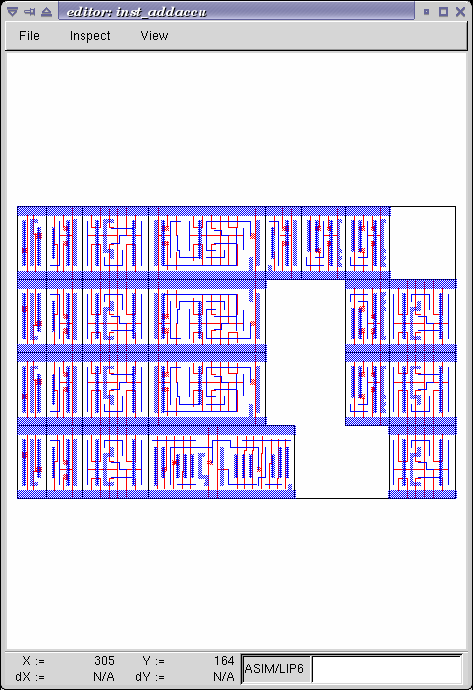
\includegraphics[width=.8\textwidth]{./images/editor.png}
\end{figure}

\newpage
\subsubsection{Function Param}

This function allows the user to give parameters when creating a cell.\\
\indent When one wants to give values to two parameters, one can type on the shell :
\begin{verbatim}
python test.py -n 4 -w 8
\end{verbatim}
\indent The file \verb-test.py- has then to contain :
\begin{verbatim}
nbit, nword = Param ( "n", "w" )
\end{verbatim}
\indent The letters typed on the shell must be the ones given as parameters of function \verb-Param-.

\subsubsection{How to instanciate your generator in another generator}

One can create a generator and instantiate it in another generator.\\
\indent To do that, the model name of the generator must have the form : "file\_name.class\_name".\\    
\indent Note that if the two generators are not in the same directory, the directory of the generator to be instantiated has to be added in the CRL\_CATA\_LIB environment variable.\\

\indent For example, in order to instanciate the addaccu created above in a cell :
\begin{verbatim}
n = 4
Generate ( "addaccu.addaccu", "my_addaccu_%dbits" % n
         , param = { 'nbit' : n } )

Inst ( "my_addaccu_%dbits" % n
     , map = { 'a'    : self.netA
             , 'b'    : self.netB
             , 'c'    : self.netC
             , 'v'    : self.netV
             , 'cmd'  : self.netCmd
             , 'cout' : self.netCout
             , 's'    : self.netS
             , 'vdd'  : self.vdd
             , 'vss'  : self.vss
             }
     )
\end{verbatim}

\begin{htmlonly}

\subsubsection{See Also}

\hyperref[ref]{\emph{Introduction}}{}{Introduction}{secintroduction}
\hyperref[ref]{\emph{Netlist}}{}{Netlist}{secnetlist}
\hyperref[ref]{\emph{Layout}}{}{Layout}{seclayout}
\hyperref[ref]{\emph{Place and Route}}{}{Place and Route}{secroute}
\hyperref[ref]{\emph{Virtual libraty}}{}{Virtual library}{seclibrary}
\hyperref[ref]{\emph{Instanciation facilities}}{}{Instanciation facilities}{secfacilities}

\end{htmlonly}

   
\section{Description of a netlist}
\label{secnetlist}
    
    \subsection{Nets}
    \label{secnet}
    \subsubsection{Name}

LogicIn, LogicOut ... -- Creation of nets

\subsubsection{Synopsys}

\begin{verbatim}
netA = LogicIn ( "a", 4 )
\end{verbatim}

\subsubsection{Description}

How to create and use nets.

\subsubsection{Nets}

Differents kind of nets are listed below :
\begin{itemize}
    \item \verb-LogicIn- : Creation of an input port
    \item \verb-LogicOut- : Creation of an output port
    \item \verb-LogicInOut- : Creation of an inout port
    \item \verb-LogicUnknown- : Creation of an input/output port which direction is not defined
    \item \verb-TriState- : Creation of a tristate port
    \item \verb-CkIn- : Creation of a clock port
    \item \verb-VddIn- : Creation of the vdd alimentation
    \item \verb-VssIn- : Creation of the vss alimentation
    \item \verb-Signal- : Creation of an internal net
\end{itemize}
        
\subsubsection{Parameters}

All kind of constructors have the same parameters :
\begin{itemize}
    \item \verb-name- : the name of the net (mandatory argument)
    \item \verb-arity- : the arity of the net (mandatory argument)
    \item \verb-indice- : for buses only : the LSB bit (optional argument : set to 0 by default)
\end{itemize}

\indent Only \verb-CkIn-, \verb-VddIn- and \verb-VssIn- do not have the same parameters : there is only the \verb-name- parameter (they are 1 bit nets).
    
\subsubsection{Example}

You can see a concrete example at : \hyperref[ref]{\emph{A concrete example}}{}{Example}{secexample}
    
\subsubsection{Errors}
    
Some errors may occur :
\begin{itemize}
    \item \verb-Error in LogicIn :-\\\verb-the lenght of the net must be a positive value.-\\One can not create a net with a negative lenght.
\end{itemize}

\subsubsection{See Also}

\hyperref[ref]{\emph{Introduction}}{}{Introduction}{secintroduction}
\hyperref[ref]{\emph{Alias}}{}{Alias}{secalias}
\hyperref[ref]{\emph{Extand}}{}{Extand}{secextend}
\hyperref[ref]{\emph{Cat}}{}{Cat}{seccat}

    \subsection{Instances}
    \label{secinst}
    \subsection{Synopsys}

\begin{verbatim}
Inst ( model
     , name
     , map = myMap
     )
\end{verbatim}

\subsection{Description}

Instantiation of an instance. The type of the instance is given by the \verb-model- parameter. The connexions are made thanks to the \verb-map- parameters.

\subsection{Parameters}

\begin{itemize}
    \item \verb-model- : Name of the mastercell of the instance to create (mandatory argument)
    \item \verb-name- : Name of the instance (optional)\\
When this argument is not defined, the instance has a name created by default. This argument is usefull when one wants to create a layout as well. Indeed, the placement of the instances is much easier when the conceptor has chosen himself the name f the instances.
    \item \verb-map- : Dictionnary for connexions in order to make the netlist\\
\end{itemize}

\subsection{Attributes}

\begin{itemize}
    \item \verb-_name- : Name of the instance (the name given as parameter if there's one, a name created otherwise)
    \item \verb-_model- : Name of the model given as argument
    \item \verb-_real_model- : Name of the model created thanks to \verb-_model- and all the parameters
    \item \verb-_map- : Dictionnary \verb-map- given at the instanciation
    \item \verb-_param- : Dictionnary \verb-param- given at the instanciation
    \item \verb-_st_cell- : The stratus cell which the instance is instanciated in
    \item \verb-_st_masterCell- : The stratus master cell of the instance\\
\end{itemize}
\indent For placement :
\begin{itemize}
    \item \verb-_plac- : tells if the instance is placed or not (UNPLACED by default)
    \item \verb-_x-, \verb-_y- : the coordinates of the instance (only for placed instances)
    \item \verb-_sym- : the symetry of the instance (only for placed instances)\\
\end{itemize}
\indent And, in connection with Hurricane :
\begin{itemize}
    \item \verb-_hur_instance- : The hurricane instance (None by default)
    \item \verb-_hur_masterCell- : The Hurricane master cell of the instance (None by default)
\end{itemize}

\subsection{Methods}

\begin{itemize}
    \item Delete : Deletion of the Hurricane instance
\end{itemize}

    \subsection{Generators}
    \label{secgen}
    \subsubsection{Name}

Generate -- Interface with the generators

\subsubsection{Synopsys}

\begin{verbatim}
Generate ( model, modelname, param = dict )
\end{verbatim}

\subsubsection{Description}

The  \verb-Generate-  function call is the generic interface to all generators.

\subsubsection{Arguments}

\begin{itemize}
    \item \verb-model- : Specifies which generator is to be invoked
    \begin{itemize}
        \item If the generator belongs to the Dpgen library provided by Stratus, the model name of the generator is simply the name of the class of the generator.
        \item If the generator is created by the user, the model name of the generator must have the form : "file\_name.class\_name". (Note that if the the generator is not in the working directory, the directory of the generator to be instantiated has to be added in the CRL\_CATA\_LIB environment variable)
    \end{itemize}
    \item \verb-modelname- : Specifies the name of the model to be generated
    \item \verb-dict- : Specifies the parameters of the generator
\end{itemize}

\subsubsection{Parameters}

Every generator has it's own parameters. They must be described in the map \verb-dict-.\\
\indent Every generator provides a netlist view. Two other views can be generated, if they are provided by the generator. Two parameters have to be given, in order to choose those views :  
\begin{itemize}
    \item 'physical' : True/False, generation of the physical view (optionnal, False by default)
    \item 'behavioral' : True/False, generation of the behavioral view (optionnal, False by default)
\end{itemize}

\begin{htmlonly}

\subsubsection{Example}

You can see a concrete example at : \hyperref[ref]{\emph{Example}}{}{Example}{secexample}

\end{htmlonly}

\subsubsection{Errors}
    
Some errors may occur :
\begin{itemize}
    \item \verb-[Stratus ERROR] Generate : the model must be described in a string.-
\end{itemize}

\begin{htmlonly}

\subsubsection{See Also}

\hyperref[ref]{\emph{Introduction}}{}{Introduction}{secintroduction}
\hyperref[ref]{\emph{Netlist}}{}{Netlist}{secnetlist}
\hyperref[ref]{\emph{Layout}}{}{Layout}{seclayout}

\end{htmlonly}

    
\section{Description of a layout}
\label{seclayout}

    \subsection{Place}
    \label{secplace}
    \subsubsection{Name}

Place -- Places an instance

\subsubsection{Synopsys}

\begin{verbatim}
Place ( ins, sym, point )
\end{verbatim}

\subsubsection{Description}

Placement of an instance.\\
\indent The instance has to be instantiated in the method \verb-Netlist-, in order to use the \verb-Place- function.
    
\subsubsection{Parameters}

\begin{itemize}
    \item \verb-ins- : Instance to place.
    \item \verb-sym- : Geometrical operation to be performed on the instance before beeing placed.\\The \verb-sym- argument can take eight legal values :
    \begin{itemize}
        \item \verb-NOSYM- : no geometrical operation is performed
        \item \verb-SYM_Y- : Y becomes -Y, that means toward X axe symetry
        \item \verb-SYM_X- : X becomes -X, that means toward Y axe symetry
        \item \verb-SYMXY- : X becomes -X, Y becomes -Y
        \item \verb-ROT_P- : a positive 90 degrees rotation takes place
        \item \verb-ROT_M- : a negative 90 degrees rotation takes place
        \item \verb-SY_RP- : Y becomes -Y, and then a positive 90 degrees rotation takes place
        \item \verb-SY_RM- : Y becomes -Y, and then a negative 90 degrees rotation takes place
    \end{itemize}
    \item \verb-point- : coordinates of the lower left corner of the abutment box of the instance in the current figure.
\end{itemize}
    
\subsubsection{Example}

\begin{verbatim}
Place ( myInst, NOSYM, XY ( 0, 0 ) )
\end{verbatim}

\subsubsection{Errors}
    
Some errors may occur :
\begin{itemize}
    \item \verb-[Stratus ERROR] Placement : the instance doesn't exist.-\\The instance must be instanciated in order to be placed.
    \item \verb-[Stratus ERROR] Placement : the first argument is not an instance.-
    \item \verb-[Stratus ERROR] Placement : the instance is already placed.-\\One can not place an instance twice
    \item \verb-[Stratus ERROR] Place : wrong argument for placement type.-\\The symetry given as argument is not correct.
    \item \verb-[Stratus ERROR] Place : wrong argument for placement,-\\\verb- the coordinates must be put in a XY object.-\\The coordinates are not descrobed the bood way.
\end{itemize}

\begin{htmlonly}
        
\subsubsection{See Also}

\hyperref[ref]{\emph{Introduction}}{}{Introduction}{secintroduction}
\hyperref[ref]{\emph{PlaceTop}}{}{PlaceTop}{sectop}
\hyperref[ref]{\emph{PlaceBottom}}{}{PlaceBottom}{secbottom}
\hyperref[ref]{\emph{PlaceRight}}{}{PlaceRight}{secright}
\hyperref[ref]{\emph{PlaceLeft}}{}{PlaceLeft}{secleft}
\hyperref[ref]{\emph{SetRefIns}}{}{SetRefIns}{secsetrefins}
\hyperref[ref]{\emph{DefAb}}{}{DefAb}{secdefab}
\hyperref[ref]{\emph{ResizeAb}}{}{ResizeAb}{secresizeab}

\end{htmlonly}

    \subsection{PlaceTop}
    \label{sectop}
    \subsubsection{Name}

PlaceTop -- Places an instance at the top of the "reference instance"

\subsubsection{Synopsys}

\begin{verbatim}
PlaceTop ( ins, sym, offsetX, offsetY )
\end{verbatim}

\subsubsection{Description}

Placement of an instance.\\
\indent The instance has to be instantiated in the method \verb-Netlist- in order to use the \verb-PlaceTop- function.\\
    
\indent The bottom left corner of the abutment box of the instance is placed, after beeing symetrized and/or rotated, toward the top left corner of the abutment box of the "reference instance". The newly placed instance becomes the "reference instance".

\subsubsection{Parameters}

\begin{itemize}
    \item \verb-ins- : Instance to place.
    \item \verb-sym- : Geometrical operation to be performed on the instance before beeing placed.\\The \verb-sym- argument can take eight legal values :
    \begin{itemize}
        \item \verb-NOSYM- : no geometrical operation is performed
        \item \verb-SYM_Y- : Y becomes -Y, that means toward X axe symetry
        \item \verb-SYM_X- : X becomes -X, that means toward Y axe symetry
        \item \verb-SYMXY- : X becomes -X, Y becomes -Y
        \item \verb-ROT_P- : a positive 90 degrees rotation takes place
        \item \verb-ROT_M- : a negative 90 degrees rotation takes place
        \item \verb-SY_RP- : Y becomes -Y, and then a positive 90 degrees rotation takes place
        \item \verb-SY_RM- : Y becomes -Y, and then a negative 90 degrees rotation takes place
    \end{itemize}
    \item \verb-offsetX- (optionnal) : An offset is put horizontally. The value given as argument must be a multiple of PITCH
    \item \verb-offsetY- (optionnal) : An offset is put vertically. The value given as argument must be a multiple of SLICE
\end{itemize}

\subsubsection{Example}

\begin{verbatim}
Place    ( myInst1, NOSYM, 0, 0 )
PlaceTop ( myInst2, SYM_Y )
\end{verbatim}

\subsubsection{Errors}
    
Some errors may occur :    
\begin{itemize}
    \item \verb-[Stratus ERROR] Placement : the instance doesn't exist.-\\The instance must be instanciated in order to be placed.
    \item \verb-[Stratus ERROR] Placement : the first argument is not an instance.-
    \item \verb-[Stratus ERROR] Placement : the instance is already placed.-\\One can not place an instance twice    
    \item \verb-[Stratus ERROR] PlaceTop : no previous instance.-\\One can use \verb-PlaceTop- only if a reference instance exist. Use a \verb-Place- call before. 
    \item \verb-[Stratus ERROR] PlaceTop : wrong argument for placement type.-\\The symetry given as argument is not correct.
\end{itemize}

\begin{htmlonly}

\subsubsection{See Also}

\hyperref[ref]{\emph{Introduction}}{}{Introduction}{secintroduction}
\hyperref[ref]{\emph{Place}}{}{Place}{secplace}
\hyperref[ref]{\emph{PlaceBottom}}{}{PlaceBottom}{secbottom}
\hyperref[ref]{\emph{PlaceRight}}{}{PlaceRight}{secright}
\hyperref[ref]{\emph{PlaceLeft}}{}{PlaceLeft}{secleft}
\hyperref[ref]{\emph{SetRefIns}}{}{SetRefIns}{secsetrefins}
\hyperref[ref]{\emph{DefAb}}{}{DefAb}{secdefab}
\hyperref[ref]{\emph{ResizeAb}}{}{ResizeAb}{secresizeab}

\end{htmlonly}

    \subsection{PlaceBottom}
    \label{secbottom}
    \subsubsection{Name}

PlaceBottom -- Places an instance below the "reference instance"

\subsubsection{Synopsys}

\begin{verbatim}
PlaceBottom ( ins, sym, offset )
\end{verbatim}

\subsubsection{Description}

Placement of an instance.\\
\indent The instance has to be instantiated in the method \verb-Netlist- in order to use the \verb-PlaceTop- function.\\
    
\indent The top left corner of the abutment box of the instance is placed, after beeing symetrized and/or rotated, toward the bottom left corner of the abutment box of the "reference instance". The newly placed instance becomes the "reference instance".

\subsubsection{Parameters}

\begin{itemize}
    \item \verb-ins- : Instance to place.
    \item \verb-sym- : Geometrical operation to be performed on the instance before beeing placed.\\The \verb-sym- argument can take eight legal values :
    \begin{itemize}
        \item \verb-NOSYM- : no geometrical operation is performed
        \item \verb-SYM_Y- : Y becomes -Y, that means toward X axe symetry
        \item \verb-SYM_X- : X becomes -X, that means toward Y axe symetry
        \item \verb-SYMXY- : X becomes -X, Y becomes -Y
        \item \verb-ROT_P- : a positive 90 degrees rotation takes place
        \item \verb-ROT_M- : a negative 90 degrees rotation takes place
        \item \verb-SY_RP- : Y becomes -Y, and then a positive 90 degrees rotation takes place
        \item \verb-SY_RM- : Y becomes -Y, and then a negative 90 degrees rotation takes place
    \end{itemize}    
    \item \verb-offset- (optionnal) : An offset is put between this instance and the reference instance. The value given as argument must be a multiple of PITCH and represents the lenght of the hole between the instances
\end{itemize}

\subsubsection{Example}

\begin{verbatim}
Place       ( myInst1, NOSYM, 0, 0 )
PlaceBottom ( myInst2, SYM_Y       )
\end{verbatim}

\subsubsection{Errors}
    
Some errors may occur :    
\begin{itemize}
    \item \verb-[Stratus ERROR] Placement : the instance doesn't exist.-\\The instance must be instanciated in order to be placed.
    \item \verb-[Stratus ERROR] Placement : the first argument is not an instance.-
    \item \verb-[Stratus ERROR] Placement : the instance is already placed.-\\One can not place an instance twice    
    \item \verb-[Stratus ERROR] PlaceBottom : no previous instance.-\\One can use \verb-PlaceTop- only if a reference instance exist. Use a \verb-Place- call before. 
    \item \verb-[Stratus ERROR] PlaceBottom : wrong argument for placement type.-\\The symetry given as argument is not correct.
\end{itemize}

\subsubsection{See Also}

\hyperref[ref]{\emph{Introduction}}{}{Introduction}{secintroduction}
\hyperref[ref]{\emph{Place}}{}{Place}{secplace}
\hyperref[ref]{\emph{PlaceTop}}{}{PlaceTop}{sectop}
\hyperref[ref]{\emph{PlaceRight}}{}{PlaceRight}{secright}
\hyperref[ref]{\emph{PlaceLeft}}{}{PlaceLeft}{secleft}
\hyperref[ref]{\emph{SetRefIns}}{}{SetRefIns}{secsetrefins}
\hyperref[ref]{\emph{DefAb}}{}{DefAb}{secdefab}
\hyperref[ref]{\emph{ResizeAb}}{}{ResizeAb}{secresizeab}

    \subsection{PlaceRight}
    \label{secright}
    \subsubsection{Name}

PlaceRight -- Places an instance at the right of the "reference instance"

\subsubsection{Synopsys}

\begin{verbatim}
PlaceRight ( ins, sym, offset )
\end{verbatim}

\subsubsection{Description}

Placement of an instance.\\
\indent The instance has to be instantiated in the method \verb-Netlist- in order to use the \verb-PlaceTop- function.\\
    
\indent The bottom left corner of the abutment box of the instance is placed, after beeing symetrized and/or rotated, toward the bottom right corner of the abutment box of the "reference instance". The newly placed instance becomes the "reference instance".

\subsubsection{Parameters}

\begin{itemize}
    \item \verb-ins- : Instance to place.
    \item \verb-sym- : Geometrical operation to be performed on the instance before beeing placed.\\The \verb-sym- argument can take eight legal values :
    \begin{itemize}
        \item \verb-NOSYM- : no geometrical operation is performed
        \item \verb-SYM_Y- : Y becomes -Y, that means toward X axe symetry
        \item \verb-SYM_X- : X becomes -X, that means toward Y axe symetry
        \item \verb-SYMXY- : X becomes -X, Y becomes -Y
        \item \verb-ROT_P- : a positive 90 degrees rotation takes place
        \item \verb-ROT_M- : a negative 90 degrees rotation takes place
        \item \verb-SY_RP- : Y becomes -Y, and then a positive 90 degrees rotation takes place
        \item \verb-SY_RM- : Y becomes -Y, and then a negative 90 degrees rotation takes place
    \end{itemize}
    \item \verb-offset- (optionnal) : An offset is put between this instance and the reference instance. The value given as argument must be a multiple of PITCH and represents the width of the hole between the instances
\end{itemize}

\subsubsection{Example}

\begin{verbatim}
Place      ( myInst1, NOSYM, 0, 0 )
PlaceRight ( myInst2, NOSYM )
\end{verbatim}

\subsubsection{Errors}
    
Some errors may occur :    
\begin{itemize}
    \item \verb-[Stratus ERROR] Placement : the instance doesn't exist.-\\The instance must be instanciated in order to be placed.
    \item \verb-[Stratus ERROR] Placement : the first argument is not an instance.-
    \item \verb-[Stratus ERROR] Placement : the instance is already placed.-\\One can not place an instance twice    
    \item \verb-[Stratus ERROR] PlaceRight : no previous instance.-\\One can use \verb-PlaceTop- only if a reference instance exist. Use a \verb-Place- call before. 
    \item \verb-[Stratus ERROR] PlaceRight : wrong argument for placement type.-\\The symetry given as argument is not correct.
\end{itemize}

\subsubsection{See Also}

\hyperref[ref]{\emph{Introduction}}{}{Introduction}{secintroduction}
\hyperref[ref]{\emph{Place}}{}{Place}{secplace}
\hyperref[ref]{\emph{PlaceTop}}{}{PlaceTop}{sectop}
\hyperref[ref]{\emph{PlaceBottom}}{}{PlaceBottom}{secbottom}
\hyperref[ref]{\emph{PlaceLeft}}{}{PlaceLeft}{secleft}
\hyperref[ref]{\emph{SetRefIns}}{}{SetRefIns}{secsetrefins}
\hyperref[ref]{\emph{DefAb}}{}{DefAb}{secdefab}
\hyperref[ref]{\emph{ResizeAb}}{}{ResizeAb}{secresizeab}

    \subsection{PlaceLeft}
    \label{secleft}
    \subsubsection{Name}

PlaceLeft -- Places an instance at the left of the "reference instance"

\subsubsection{Synopsys}

\begin{verbatim}
PlaceLeft ( ins, sym, offset )
\end{verbatim}

\subsubsection{Description}

Placement of an instance.\\
\indent The instance has to be instantiated in the method \verb-Netlist- in order to use the \verb-PlaceTop- function.\\
    
\indent The bottom right corner of the abutment box of the instance is placed, after beeing symetrized and/or rotated, toward the bottom left corner of the abutment box of the "reference instance". The newly placed instance becomes the "reference instance".

\subsubsection{Parameters}

\begin{itemize}
    \item \verb-ins- : Instance to place.
    \item \verb-sym- : Geometrical operation to be performed on the instance before beeing placed.\\The \verb-sym- argument can take eight legal values :
    \begin{itemize}
        \item \verb-NOSYM- : no geometrical operation is performed
        \item \verb-SYM_Y- : Y becomes -Y, that means toward X axe symetry
        \item \verb-SYM_X- : X becomes -X, that means toward Y axe symetry
        \item \verb-SYMXY- : X becomes -X, Y becomes -Y
        \item \verb-ROT_P- : a positive 90 degrees rotation takes place
        \item \verb-ROT_M- : a negative 90 degrees rotation takes place
        \item \verb-SY_RP- : Y becomes -Y, and then a positive 90 degrees rotation takes place
        \item \verb-SY_RM- : Y becomes -Y, and then a negative 90 degrees rotation takes place
    \end{itemize}
    \item \verb-offset- (optionnal) : An offset is put between this instance and the reference instance. The value given as argument must be a multiple of PITCH and represents the width of the hole between the instances    
\end{itemize}

\subsubsection{Example}

\begin{verbatim}
Place     ( myInst1, NOSYM, 0, 0 )
PlaceLeft ( myInst2, NOSYM )
\end{verbatim}

\subsubsection{Errors}
    
Some errors may occur :    
\begin{itemize}
    \item \verb-[Stratus ERROR] Placement : the instance doesn't exist.-\\The instance must be instanciated in order to be placed.
    \item \verb-[Stratus ERROR] Placement : the first argument is not an instance.-
    \item \verb-[Stratus ERROR] Placement : the instance is already placed.-\\One can not place an instance twice    
    \item \verb-[Stratus ERROR] PlaceLeft : no previous instance.-\\One can use \verb-PlaceTop- only if a reference instance exist. Use a \verb-Place- call before. 
    \item \verb-[Stratus ERROR] PlaceLeft : wrong argument for placement type.-\\The symetry given as argument is not correct.
\end{itemize}

\subsubsection{See Also}

\hyperref[ref]{\emph{Introduction}}{}{Introduction}{secintroduction}
\hyperref[ref]{\emph{Place}}{}{Place}{secplace}
\hyperref[ref]{\emph{PlaceTop}}{}{PlaceTop}{sectop}
\hyperref[ref]{\emph{PlaceBottom}}{}{PlaceBottom}{secbottom}
\hyperref[ref]{\emph{PlaceRight}}{}{PlaceRight}{secright}
\hyperref[ref]{\emph{SetRefIns}}{}{SetRefIns}{secsetrefins}
\hyperref[ref]{\emph{DefAb}}{}{DefAb}{secdefab}
\hyperref[ref]{\emph{ResizeAb}}{}{ResizeAb}{secresizeab}

    \subsection{SetRefIns}
    \label{secsetrefins}
    \subsubsection{Name}

SetRefIns -- Defines the new "reference instance" for placement

\subsubsection{Synopsys}

\begin{verbatim}
SetRefIns ( ins )
\end{verbatim}

\subsubsection{Description}

This function defines the new "reference instance", used as starting point in the relative placement functions.\\
\indent It's regarding the abutmentbox of the instance \verb-ins- that the next instance is going to be placed, if using the appropriate functions.\\
    
\indent Note that the more recently placed instance becomes automaticaly the "reference instance", if SetRefIns isn't called.
    
\subsubsection{Parameters}

\begin{itemize}
    \item \verb-ins- : defines the new "reference instance"
\end{itemize}
    
\subsubsection{Example}

\begin{verbatim}
Place      ( myInst1, NOSYM, 0, 0 )
PlaceRight ( myInst2, NOSYM       )

SetRefIns  ( myInst1 )
PlaceTop   ( myInst3, SYM_Y       )
\end{verbatim}

\indent \verb-myInst3- is on top of \verb-myInst1- instead of \verb-myInst2-.

\subsubsection{Errors}
    
Some errors may occur :
\begin{itemize}
    \item \verb-[Stratus ERROR] SetRefIns : the instance doesn't exist.-\\If the instance has not been instanciated, it is impossible do to any placement from it.
    \item \verb-[Stratus ERROR] SetRefIns : the instance ...is not placed.-\\If the instance has not been placed, it is impossible do to any placement from it.
\end{itemize}
         
\subsubsection{See Also}

\hyperref[ref]{\emph{Introduction}}{}{Introduction}{secintroduction}
\hyperref[ref]{\emph{Place}}{}{Place}{secplace}
\hyperref[ref]{\emph{PlaceTop}}{}{PlaceTop}{sectop}
\hyperref[ref]{\emph{PlaceBottom}}{}{PlaceBottom}{secbottom}
\hyperref[ref]{\emph{PlaceRight}}{}{PlaceRight}{secright}
\hyperref[ref]{\emph{PlaceLeft}}{}{PlaceLeft}{secleft}
\hyperref[ref]{\emph{DefAb}}{}{DefAb}{secdefab}
\hyperref[ref]{\emph{ResizeAb}}{}{ResizeAb}{secresizeab}

    \subsection{DefAb}
    \label{secdefab}
    \subsubsection{Name}

DefAb -- Creates the abutment box of the current cell

\subsubsection{Synopsys}
      
\begin{verbatim}
DefAb ( x1, y1, x2, y2 )
\end{verbatim}
    
\subsubsection{Description}

This function creates the abutment box of the current cell.\\
         
\indent Note that one does not have to call this function before saving in order to create the abutment box. The abutment box is created nevertheless (given to placed instances). This function is usefull if one wants to create an abutment before placing the instances.

\subsubsection{Parameters}

\begin{itemize}
    \item \verb-( x1, y1)- : coordinates of the bottom left corner of the created abutment box.
    \item \verb-( x2, y2)- : coordinates of the top right corner of the created abutment box.
\end{itemize}
    
\subsubsection{Example}

\begin{verbatim}
DefAb ( 0, 0, 500, 100 )
    
Place ( Inv, NOSYM, 0, 0 )
\end{verbatim}

\subsubsection{Errors}
    
Some errors may occur :
\begin{itemize}
    \item \verb-[Stratus ERROR] DefAb : an abutment box already exists.-\\\verb- Maybe you should use ResizeAb function.-\\One has called DefAb but the current cell already has an abutment box.\\In order to modify the current abutment box, the function to call is ResizeAb.
    \item \verb-[Stratus ERROR] DefAb :-\\\verb-Coordinates of an abutment Box in y must be multiple of the slice.-\\\verb-Coordinates of an abutment Box in x must be multiple of the pitch.-\\One has called DefAb with non authorized values.
\end{itemize}

\subsubsection{See Also}

\hyperref[ref]{\emph{Introduction}}{}{Introduction}{secintroduction}
\hyperref[ref]{\emph{Place}}{}{Place}{secplace}
\hyperref[ref]{\emph{PlaceTop}}{}{PlaceTop}{sectop}
\hyperref[ref]{\emph{PlaceBottom}}{}{PlaceBottom}{secbottom}
\hyperref[ref]{\emph{PlaceRight}}{}{PlaceRight}{secright}
\hyperref[ref]{\emph{PlaceLeft}}{}{PlaceLeft}{secleft}
\hyperref[ref]{\emph{SetRefIns}}{}{SetRefIns}{secsetrefins}
\hyperref[ref]{\emph{ResizeAb}}{}{ResizeAb}{secresizeab}

    \subsection{ResizeAb}
    \label{secresizeab}
    \subsubsection{Name}

ResizeAb -- Modifies the abutment box of the current cell

\subsubsection{Synopsys}

\begin{verbatim}
ResizeAb ( dx1, dy1, dx2, dy2 )
\end{verbatim}

\subsubsection{Description}

This function modifies the abutment box of the current cell.\\
\indent The coordinates of the abutment box are the coordinates of the envelop of the abutment boxes of each instance plus the delta values given as argument.\\

\indent Note that one can not call this function in order to create the abutment box. This fonction only modifies the already created abutment box.
    
\subsubsection{Parameters}

\begin{itemize}
    \item \verb-(dx1, dy1)- : Values to be substracted to the lower left corner of the previous abutment box.
    \item \verb-(dx2, dy2)- : Values to be added to the upper right corner of the previous abutment box.
\end{itemize}

\indent The Values are used as follow :
\begin{figure}[h!]
\centering
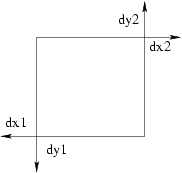
\includegraphics[width=.3\textwidth]{./images/resizeAb}
\end{figure}
      
\subsubsection{Example}

\begin{verbatim}
% Expansion of the abutment box at the top and the bottom
ResizeAb ( 0, 100, 0, 100 )
\end{verbatim}

\subsubsection{Errors}
    
Some errors may occur :
\begin{itemize}
    \item \verb- [Stratus ERROR] ResizeAb :-\\\verb-Coordinates of an abutment Box in y must be multiple of the slice.-\\\verb-Coordinates of an abutment Box in x must be multiple of the pitch.-\\One has called ResizeAb with non authorized values
    \item \verb- [Stratus ERROR] ResizeAb :-\\\verb-one of the values of dx1 or dx2 (dy1 or dy2)  is incompatible with-\\\verb-the size of the abutment box.-\\\verb-Coordinates of an abutment Box in x must be multiple of the pitch.-\\One has called ResizeAb with a value which deteriorates the abtument box
\end{itemize}

\begin{htmlonly}

\subsubsection{See Also}

\hyperref[ref]{\emph{Introduction}}{}{Introduction}{secintroduction}
\hyperref[ref]{\emph{Place}}{}{Place}{secplace}
\hyperref[ref]{\emph{PlaceTop}}{}{PlaceTop}{sectop}
\hyperref[ref]{\emph{PlaceBottom}}{}{PlaceBottom}{secbottom}
\hyperref[ref]{\emph{PlaceRight}}{}{PlaceRight}{secright}
\hyperref[ref]{\emph{PlaceLeft}}{}{PlaceLeft}{secleft}
\hyperref[ref]{\emph{SetRefIns}}{}{SetRefIns}{secsetrefins}
\hyperref[ref]{\emph{DefAb}}{}{DefAb}{secdefab}

\end{htmlonly}

    
\section{Place and Route}
\label{secroute}

    \subsection{PlaceSegment}
    \label{secsegment}
    \subsubsection{Name}

PlaceSegment -- Places a segment

\subsubsection{Synopsys}

\begin{verbatim}
PlaceSegment ( net, layer, point1, point2, width )
\end{verbatim}

\subsubsection{Description}

Placement of a segment.\\
\indent The segment is created between \verb-point1- and \verb-point2- on the layer \verb-layer- and with width \verb-width-. It belongs to the net \verb-net-.\\
\indent Note that the segment must be horizontal or vertival.
    
\subsubsection{Parameters}

\begin{itemize}
    \item \verb-net- : Net which the segment belongs to
    \item \verb-layer- : Layer of the segment.\\The \verb-layer- argument is a string wich can take different values, thanks to the technology (file described in HUR\_TECHNO\_NAME)
    \begin{itemize}
        \item NWELL, PWELL, ptie, ntie, pdif, ndif, ntrans, ptrans, poly, ALU1, ALU2, ALU3, ALU4, ALU5, ALU6, VIA1, VIA2, VIA3, VIA4, VIA5, TEXT, UNDEF, SPL1, TALU1, TALU2, TALU3, TALU4, TALU5, TALU6, POLY, NTIE, PTIE, NDIF, PDIF, PTRANS, NTRANS, CALU1, CALU2, CALU3, CALU4, CALU5, CALU6, CONT\_POLY, CONT\_DIF\_N, CONT\_DIF\_P, CONT\_BODY\_N, CONT\_BODY\_P, via12, via23, via34, via45, via56, via24, via25, via26, via35, via36, via46, CONT\_TURN1, CONT\_TURN2, CONT\_TURN3, CONT\_TURN4, CONT\_TURN5, CONT\_TURN6
    \end{itemize}
    \item \verb-point1-, \verb-point2- : The segment is created between those two points
\end{itemize}
    
\subsubsection{Example}

\begin{verbatim}
PlaceSegment ( myNet, "ALU3", XY (10, 0), XY (10, 100), 2 )
\end{verbatim}

\subsubsection{Errors}
    
Some errors may occur :
\begin{itemize}
    \item \verb-[Stratus ERROR] PlaceSegment : Argument layer must be a string.-
    \item \verb-[Stratus ERROR] PlaceSegment : Wrong argument,-\\\verb-the coordinates of the segment must be put in XY objects.-
    \item \verb-[Stratus ERROR] PlaceSegment : Segments are vertical or horizontal.-\\The two references given as argument do not describe a vertical or horizontal segment. Wether coordinate x or y of the references must be identical. 
\end{itemize}

\begin{htmlonly}
        
\subsubsection{See Also}

\hyperref[ref]{\emph{Introduction}}{}{Introduction}{secintroduction}
\hyperref[ref]{\emph{Layout}}{}{Layout}{seclayout}
\hyperref[ref]{\emph{PlaceContact}}{}{PlaceContact}{seccontact}
\hyperref[ref]{\emph{PlacePin}}{}{PlacePin}{secpin}
\hyperref[ref]{\emph{PlaceRef}}{}{PlaceRef}{secref}
\hyperref[ref]{\emph{GetRefXY}}{}{GetRefXY}{secgetref}
\hyperref[ref]]{\emph{CopyUpSegment}}{}{CopyUpSegment}{seccopy}

\end{htmlonly}

    \subsection{PlaceContact}
    \label{seccontact}
    \subsubsection{Name}

PlaceContact -- Places a contact

\subsubsection{Synopsys}

\begin{verbatim}
PlaceContact ( net, layer, point, width, height )
\end{verbatim}

\subsubsection{Description}

Placement of a contact.\\
\indent The contact is located at the coodinates of \verb-point-, on the layer \verb-layer- and has a size of 1 per 1. It belongs to the net \verb-net-.\\
\indent Note that the segment must be horizontal or vertival.
    
\subsubsection{Parameters}

\begin{itemize}
    \item \verb-net- : Net which the contact belongs to
    \item \verb-layer- : Layer of the segment.\\The \verb-layer- argument is a string wich can take different values, thanks to the technology (file described in HUR\_TECHNO\_NAME)
    \begin{itemize}
        \item NWELL, PWELL, ptie, ntie, pdif, ndif, ntrans, ptrans, poly, ALU1, ALU2, ALU3, ALU4, ALU5, ALU6, VIA1, VIA2, VIA3, VIA4, VIA5, TEXT, UNDEF, SPL1, TALU1, TALU2, TALU3, TALU4, TALU5, TALU6, POLY, NTIE, PTIE, NDIF, PDIF, PTRANS, NTRANS, CALU1, CALU2, CALU3, CALU4, CALU5, CALU6, CONT\_POLY, CONT\_DIF\_N, CONT\_DIF\_P, CONT\_BODY\_N, CONT\_BODY\_P, via12, via23, via34, via45, via56, via24, via25, via26, via35, via36, via46, CONT\_TURN1, CONT\_TURN2, CONT\_TURN3, CONT\_TURN4, CONT\_TURN5, CONT\_TURN6
    \end{itemize}
    \item \verb-point- : Coodinates of the contact
    \item \verb-width- : Width of the contact
    \item \verb-height- : Height of the contact
\end{itemize}
    
\subsubsection{Example}

\begin{verbatim}
PlaceContact ( myNet, "ALU2", XY (10, 0), 2, 2 )
\end{verbatim}

\subsubsection{Errors}
    
Some errors may occur :
\begin{itemize}
    \item \verb-[Stratus ERROR] PlaceContact : Argument layer must be a string.-
    \item \verb-[Stratus ERROR] PlaceContact : Wrong argument,-\\\verb-the coordinates of the contact must be put in a XY object.-
\end{itemize}

\begin{htmlonly}

\subsubsection{See Also}

\hyperref[ref]{\emph{Introduction}}{}{Introduction}{secintroduction}
\hyperref[ref]{\emph{Layout}}{}{Layout}{seclayout}
\hyperref[ref]{\emph{PlaceSegment}}{}{PlaceSegment}{secsegment}
\hyperref[ref]{\emph{PlacePin}}{}{PlacePin}{secpin}
\hyperref[ref]{\emph{PlaceRef}}{}{PlaceRef}{secref}
\hyperref[ref]{\emph{GetRefXY}}{}{GetRefXY}{secgetref}
\hyperref[ref]{\emph{CopyUpSegment}}{}{CopyUpSegment}{seccopy}

\end{htmlonly}

    \subsection{PlacePin}
    \label{secpin}
    \subsubsection{Name}

PlacePin -- Places a pin

\subsubsection{Synopsys}

\begin{verbatim}
PlacePin ( net, layer, direction, point, width, height )
\end{verbatim}

\subsubsection{Description}

Placement of a pin.\\
\indent The pin is located at the coodinates of \verb-point-, on the layer \verb-layer-, has a a direction of \verb-direction- and size of 1 per 1. It belongs to the net \verb-net-.
    
\subsubsection{Parameters}

\begin{itemize}
    \item \verb-net- : Net which the pin belongs to
    \item \verb-layer- : Layer of the segment.\\The \verb-layer- argument is a string wich can take different values, thanks to the technology (file described in HUR\_TECHNO\_NAME)
    \begin{itemize}
        \item NWELL, PWELL, ptie, ntie, pdif, ndif, ntrans, ptrans, poly, ALU1, ALU2, ALU3, ALU4, ALU5, ALU6, VIA1, VIA2, VIA3, VIA4, VIA5, TEXT, UNDEF, SPL1, TALU1, TALU2, TALU3, TALU4, TALU5, TALU6, POLY, NTIE, PTIE, NDIF, PDIF, PTRANS, NTRANS, CALU1, CALU2, CALU3, CALU4, CALU5, CALU6, CONT\_POLY, CONT\_DIF\_N, CONT\_DIF\_P, CONT\_BODY\_N, CONT\_BODY\_P, via12, via23, via34, via45, via56, via24, via25, via26, via35, via36, via46, CONT\_TURN1, CONT\_TURN2, CONT\_TURN3, CONT\_TURN4, CONT\_TURN5, CONT\_TURN6
    \end{itemize}
    \item \verb-direction- : Direction of the pin
    \begin{itemize}
        \item UNDEFINED, NORTH, SOUTH, EAST, WEST
    \end{itemize}
    \item \verb-point- : Coodinates of the pin
    \item \verb-width- : Width of the pin
    \item \verb-height- : Height of the pin
\end{itemize}
    
\subsubsection{Example}

\begin{verbatim}
PlacePin ( myNet, "ALU2", NORTH, XY (10, 0), 2, 2 )
\end{verbatim}

\subsubsection{Errors}
    
Some errors may occur :
\begin{itemize}
    \item \verb-[Stratus ERROR] PlacePin : Argument layer must be a string.-
    \item \verb-[Stratus ERROR] PlacePin : Illegal pin access direction.-\\\verb-The values are : UNDEFINED, NORTH, SOUTH, EAST, WEST.-
    \item \verb-[Stratus ERROR] PlacePin : Wrong argument,-\\\verb-the coordinates of the pin must be put in a XY object.-
\end{itemize}

\begin{htmlonly}
        
\subsubsection{See Also}

\hyperref[ref]{\emph{Introduction}}{}{Introduction}{secintroduction}
\hyperref[ref]{\emph{Layout}}{}{Layout}{seclayout}
\hyperref[ref]{\emph{PlaceSegment}}{}{PlaceSegment}{secsegment}
\hyperref[ref]{\emph{PlaceContact}}{}{PlaceContact}{seccontact}
\hyperref[ref]{\emph{PlaceRef}}{}{PlaceRef}{secref}
\hyperref[ref]{\emph{GetRefXY}}{}{GetRefXY}{secgetref}
\hyperref[ref]{\emph{CopyUpSegment}}{}{CopyUpSegment}{seccopy}

\end{htmlonly}
    
    \subsection{PlaceRef}
    \label{secref}
    \subsubsection{Name}

PlaceRef -- Places a reference

\subsubsection{Synopsys}

\begin{verbatim}
PlaceRef ( point, name )
\end{verbatim}

\subsubsection{Description}

Placement of a reference.\\
\indent The reference is located at the coordinates of \verb-point-, with name \verb-name-.
    
\subsubsection{Parameters}

\begin{itemize}
    \item \verb-point- : Coodinates of the reference
    \item \verb-name- : Name of the reference
\end{itemize}
    
\subsubsection{Example}

\begin{verbatim}
PlaceRef ( XY (10, 0), "myref" )
\end{verbatim}

\subsubsection{Errors}
    
Some errors may occur :
\begin{itemize}
    \item \verb-[Stratus ERROR] PlaceRef : Wrong argument,-\\\verb-the coordinates of the reference must be put in a XY object.-
    \item \verb-[Stratus ERROR] PlaceRef : Argument layer must be a string.-
\end{itemize}

\begin{htmlonly}
        
\subsubsection{See Also}

\hyperref[ref]{\emph{Introduction}}{}{Introduction}{secintroduction}
\hyperref[ref]{\emph{Layout}}{}{Layout}{seclayout}
\hyperref[ref]{\emph{PlaceSegment}}{}{PlaceSegment}{secsegment}
\hyperref[ref]{\emph{PlaceContact}}{}{PlaceContact}{seccontact}
\hyperref[ref]{\emph{PlacePin}}{}{PlacePin}{secpin}
\hyperref[ref]{\emph{GetRefXY}}{}{GetRefXY}{secgetref}
\hyperref[ref]{\emph{CopyUpSegment}}{}{CopyUpSegment}{seccopy}

\end{htmlonly}

    \subsection{GetRefXY}
    \label{secgetref}
    \subsubsection{Name}

GetRefXY -- Returns the coordinates of a reference

\subsubsection{Synopsys}

\begin{verbatim}
GetRefXY ( pathname, refname )
\end{verbatim}

\subsubsection{Description}

Computation of coordinates.\\
\indent The point returned (object XY) represents the location of the reference of name \verb-refname-  within the coodinates system of the top cell. The reference \verb-refname- is instanciated in an instance found thanks to \verb-pathname- which represents an ordered sequence of instances through the hierarchy.
    
\subsubsection{Parameters}

\begin{itemize}
    \item \verb-pathname- : The path in order to obtain, from the top cell, the instance the reference \verb-refname- belongs to
    \item \verb-refname- : The name of the reference
\end{itemize}
    
\subsubsection{Example}

\indent The cell which is being created (the top cell), instanciates a generator with instance name "my\_dpgen\_and2". This generator instanciates an instance called "cell\_1" which the reference "i0\_20" belongs to.
\begin{verbatim}
GetRefXY ( "my_dpgen_and2.cell_1", "i0_20" )
\end{verbatim}

\subsubsection{Errors}
    
Some errors may occur :
\begin{itemize}
    \item \verb-[Stratus ERROR] GetRefXY :-\\\verb-The instance's path must be put with a string.-
    \item \verb-[Stratus ERROR] GetRefXY :-\\\verb-The reference must be done with it's name : a string.-
    \item \verb-[Stratus ERROR] GetRefXY :-\\\verb-No reference found with name ... in masterCell ...-
\end{itemize}

\begin{htmlonly}

\subsubsection{See Also}

\hyperref[ref]{\emph{Introduction}}{}{Introduction}{secintroduction}
\hyperref[ref]{\emph{Layout}}{}{Layout}{seclayout}
\hyperref[ref]{\emph{PlaceSegment}}{}{PlaceSegment}{secsegment}
\hyperref[ref]{\emph{PlaceContact}}{}{PlaceContact}{seccontact}
\hyperref[ref]{\emph{PlacePin}}{}{PlacePin}{secpin}
\hyperref[ref]{\emph{PlaceRef}}{}{PlaceRef}{secref}
\hyperref[ref]{\emph{CopyUpSegment}}{}{CopyUpSegment}{seccopy}

\end{htmlonly}

    \subsection{CopyUpSegment}
    \label{seccopy}
    \subsubsection{Name}

CopyUpSegment -- Copies the segment of an instance in the current cell

\subsubsection{Synopsys}

\begin{verbatim}
CopyUpSegment ( pathname, netname, newnet  )
\end{verbatim}

\subsubsection{Description}

Duplication of a segment.\\
\indent The segment is created with the same cordinates and layer as the segment corresponding to the net \verb-netname- in the instance found thanks to \verb-pathname-. It belongs to the net \verb-newnet-.\\
\indent Note that if several segments correspond to the net, they are all going to be copied.
    
\subsubsection{Parameters}

\begin{itemize}
    \item \verb-pathname- : The path in order to obtain, from the top cell, the instance the net \verb-netname- belongs to
    \item \verb-netname- : The name of the net which the segment belongs to
    \item \verb-net- : The net which the top cell segment os going to belong to
\end{itemize}
    
\subsubsection{Example}

\begin{verbatim}
CopuUpSegment ( "my_dpgen_and2.cell_1", "i0", myNet )
\end{verbatim}

\subsubsection{Errors}
    
Some errors may occur :
\begin{itemize}
    \item \verb-[Stratus ERROR] CopyUpSegment :-\\\verb-The instance's path must be put with a string.-
    \item \verb-[Stratus ERROR] CopyUpSegment :-\\\verb-The segment must be done with it's name : a string.-
    \item \verb-[Stratus ERROR] CopyUpSegment :-\\\verb-No net found with name ... in masterCell ...-\\There is no net with name \verb-netname- in the instance found thanks to the path \verb-pathname-.
    \item \verb-[Stratus ERROR] CopyUpSegment :-\\\verb-No segment found with net ... in masterCell ...-\\The net with name \verb-netname- has no segment. So the copy of segment can not be done.
    \item \verb-[Stratus ERROR] CopyUpSegment :-\\\verb-the segment of net ... are not of type CALU.-\\In other words, the net is not an external net. The copy can be done only with external nets.
\end{itemize}

\begin{htmlonly}

\subsubsection{See Also}

\hyperref[ref]{\emph{Introduction}}{}{Introduction}{secintroduction}
\hyperref[ref]{\emph{Layout}}{}{Layout}{seclayout}
\hyperref[ref]{\emph{PlaceSegment}}{}{PlaceSegment}{secsegment}
\hyperref[ref]{\emph{PlaceContact}}{}{PlaceContact}{seccontact}
\hyperref[ref]{\emph{PlacePin}}{}{PlacePin}{secpin}
\hyperref[ref]{\emph{PlaceRef}}{}{PlaceRef}{secref}
\hyperref[ref]{\emph{GetRefXY}}{}{GetRefXY}{secgetref}

\end{htmlonly}
    
    \subsection{PlaceCentric}
    \label{seccentric}
    \subsubsection{Name}

PlaceCentric -- Placement of an instance in the middle of an abutment box

\subsubsection{Synopsys}

\begin{verbatim}
PlaceCentric ( ins )
\end{verbatim}

\subsubsection{Description}

This function places an instance in the middle of and abutment box.\\
\indent The instance has to be instantiated in the method \verb-Netlist- in order to use this function.
    
\subsubsection{Parameters}

\begin{itemize}
    \item \verb-ins- : Instance to place
\end{itemize}

%\subsubsection{Example}
%
%\begin{verbatim}
%PlaceCentric ( core )
%\end{verbatim}
%
\subsubsection{Errors}
    
Some errors may occur :
\begin{itemize}
    \item \verb-[Stratus ERROR] PlaceCentric: the instance does not exist.-\\The instance must be instanciated in order to be placed.
    \item \verb-[Stratus ERROR] PlaceCentric :-\\\verb-the instance's size is greater than this model.-\\The instance must fit in the abutment box. The abutment box may not be big enough.
\end{itemize}

\begin{htmlonly}

\subsubsection{See Also}

\hyperref[ref]{\emph{Introduction}}{}{Introduction}{secintroduction}
\hyperref[ref]{\emph{Layout}}{}{Layout}{seclayout}
\hyperref[ref]{\emph{PlaceGlu}}{}{PlaceGlu}{secglu}
\hyperref[ref]{\emph{FillCell}}{}{FillCell}{secfillcell}
\hyperref[ref]{\emph{Pads}}{}{Pads}{secpads}
\hyperref[ref]{\emph{Alimentation rails}}{}{Alimentation rails}{secrails}
\hyperref[ref]{\emph{Alimentation connectors}}{}{Alimentation connectors}{secconnectors}
\hyperref[ref]{\emph{PowerRing}}{}{PowerRing}{secpowerring}
\hyperref[ref]{\emph{RouteCk}}{}{RouteCk}{secrouteck}

\end{htmlonly}

    \subsection{PlaceGlu}
    \label{secglu}
    \subsubsection{Name}

PlaceGlue -- Automatic placement of non placed instances

\subsubsection{Synopsys}

\begin{verbatim}
PlaceGlue ( cell )
\end{verbatim}

\subsubsection{Description}

This function places, thanks to the automatic placer Mistral of Coriolis, all the non placed instances of the cell.
    
\subsubsection{Parameters}

\begin{itemize}
    \item \verb-cell- : the cell which the fonction is applied to
\end{itemize}
    
%\subsubsection{Example}
%
%\begin{verbatim}
%PlaceGlue ( core )
%\end{verbatim}
%
\subsubsection{See Also}

\hyperref[ref]{\emph{Introduction}}{}{Introduction}{secintroduction}
\hyperref[ref]{\emph{Layout}}{}{Layout}{seclayout}
\hyperref[ref]{\emph{PlaceCentric}}{}{PlaceCentric}{seccentric}
\hyperref[ref]{\emph{FillCell}}{}{FillCell}{secfillcell}
\hyperref[ref]{\emph{Pads}}{}{Pads}{secpads}
\hyperref[ref]{\emph{Alimentation rails}}{}{Alimentation rails}{secrails}
\hyperref[ref]{\emph{Alimentation connectors}}{}{Alimentation connectors}{secconnectors}
\hyperref[ref]{\emph{PowerRing}}{}{PowerRing}{secpowerring}
\hyperref[ref]{\emph{RouteCk}}{}{RouteCk}{secrouteck}

    \subsection{FillCell}
    \label{secfillcell}
    \subsubsection{Name}

FillCell -- Automatic placement of ties.

\subsubsection{Synopsys}

\begin{verbatim}
FillCell ( cell )
\end{verbatim}

\subsubsection{Description}

This function places automatically ties.
    
\subsubsection{Parameters}

\begin{itemize}
    \item \verb-cell- : the cell which the fonction is applied to
\end{itemize}
    
%\subsubsection{Example}
%
%\begin{verbatim}
%FillCell ( core )
%\end{verbatim}
%
\subsubsection{Errors}
    
Some errors may occur :
\begin{itemize}
    \item \verb-[Stratus ERROR] FillCell : Given cell doesn't exist.-\\The argument is wrong. Check if one has created the cell correctly.
\end{itemize}

\begin{htmlonly}

\subsubsection{See Also}

\hyperref[ref]{\emph{Introduction}}{}{Introduction}{secintroduction}
\hyperref[ref]{\emph{Layout}}{}{Layout}{seclayout}
\hyperref[ref]{\emph{PlaceCentric}}{}{PlaceCentric}{seccentric}
\hyperref[ref]{\emph{PlaceGlu}}{}{PlaceGlu}{secglu}
\hyperref[ref]{\emph{Pads}}{}{Pads}{secpads}
\hyperref[ref]{\emph{Alimentation rails}}{}{Alimentation rails}{secrails}
\hyperref[ref]{\emph{Alimentation connectors}}{}{Alimentation connectors}{secconnectors}
\hyperref[ref]{\emph{PowerRing}}{}{PowerRing}{secpowerring}
\hyperref[ref]{\emph{RouteCk}}{}{RouteCk}{secrouteck}

\end{htmlonly}

    \subsection{Pads}
    \label{secpads}
    \subsubsection{Name}

PadNorth, PadSouth, PadEast, PasWest -- Placement of pads at the periphery of the cell

\subsubsection{Synopsys}

\begin{verbatim}
PadNorth ( args )
\end{verbatim}

\subsubsection{Description}

These functions place the pads given as arguments at the given side of the cell (PadNorth : up north, PadSouth : down south ...).
Pads are placed from bottom to top for PadNorth and PadSouth and from left to right for PadWest and PasEast.
    
\subsubsection{Parameters}

\begin{itemize}
    \item \verb-args- : List of pads to be placed
\end{itemize}

\subsubsection{Example}

\begin{verbatim}
PadSouth ( self.p_cin, self.p_np, self.p_ng, self.p_vssick0
         , self.p_vddeck0, self.p_vsseck1, self.p_vddeck1, self.p_cout
         , self.p_y[0], self.p_y[1], self.p_y[2]
         )
\end{verbatim}

\subsubsection{Errors}

Some errors may occur :
\begin{itemize}
    \item \verb-[Stratus ERROR] PadNorth : not enough space for all pads.-\\The abutment box is not big enough in order to place all the pads. Maybe one could put pads on other faces of the cell.
    \item \verb-[Stratus ERROR] PadNorth : one instance doesn't exist.-\\One of the pads given as arguments does not exist
    \item \verb-[Stratus ERROR] PadNorth : one argument is not an instance.-\\One of the pads is not one of the pads of the cell.
    \item \verb-[Stratus ERROR] PadNorth : the instance ins is already placed.-\\One is trying to place a pad twice.
    \item \verb-[Stratus ERROR] PadNorth : pad ins must be closer to the center.-\\The pad name ins must be put closer to the center in order to route the cell
\end{itemize}

\begin{htmlonly}

\subsubsection{See Also}

\hyperref[ref]{\emph{Introduction}}{}{Introduction}{secintroduction}
\hyperref[ref]{\emph{Layout}}{}{Layout}{seclayout}
\hyperref[ref]{\emph{PlaceCentric}}{}{PlaceCentric}{seccentric}
\hyperref[ref]{\emph{PlaceGlu}}{}{PlaceGlu}{secglu}
\hyperref[ref]{\emph{FillCell}}{}{FillCell}{secfillcell}
\hyperref[ref]{\emph{Alimentation rails}}{}{Alimentation rails}{secrails}
\hyperref[ref]{\emph{Alimentation connectors}}{}{Alimentation connectors}{secconnectors}
\hyperref[ref]{\emph{PowerRing}}{}{PowerRing}{secpowerring}
\hyperref[ref]{\emph{RouteCk}}{}{RouteCk}{secrouteck}

\end{htmlonly}

    \subsection{Alimentation rails}
    \label{secrails}
    \subsubsection{Name}

AlimVerticalRail, AlimHorizontalRail -- Placement of a vertical/horizontal alimentation call back

\subsubsection{Synopsys}

\begin{verbatim}
AlimVerticalRail ( nb )
\end{verbatim}

\subsubsection{Description}

These functions place a vertical/horizontal alimentation call back. It's position is given by the parameter given.
    
\subsubsection{Parameters}

\begin{itemize}
    \item \verb-nb- : coordinate of the rail
    \begin{itemize}
        \item For AlimVerticalRail, \verb-nb- is in pitches i.e. 5 lambdas
        \item For AlimHorizontalRail, \verb-nb- is in slices i.e. 50 lambdas
    \end{itemize}
\end{itemize}
    
\subsubsection{Example}

\begin{verbatim}
AlimVerticalRail   (  50 )
AlimVerticalRail   ( 150 )
    
AlimHorizontalRail (  10 )
\end{verbatim}

\subsubsection{Errors}
    
Some errors may occur :
\begin{itemize}
    \item \verb-[Stratus ERROR] AlimHorizontalRail :-\\\verb-Illegal argument y, y must be between ... and ...-\\The argument given is wrong : the call back would not be in the abutment box.
    \item \verb-[Stratus ERROR] Placement of cells :-\\\verb-please check your file of layout with DRUC.-\\The placement of the cell needs to be correct in order to place a call back. Check the errors of placement.
\end{itemize} 

\subsubsection{See Also}

\hyperref[ref]{\emph{Introduction}}{}{Introduction}{secintroduction}
\hyperref[ref]{\emph{Layout}}{}{Layout}{seclayout}
\hyperref[ref]{\emph{PlaceCentric}}{}{PlaceCentric}{seccentric}
\hyperref[ref]{\emph{PlaceGlu}}{}{PlaceGlu}{secglu}
\hyperref[ref]{\emph{FillCell}}{}{FillCell}{secfillcell}
\hyperref[ref]{\emph{Pads}}{}{Pads}{secpads}
\hyperref[ref]{\emph{Alimentation connectors}}{}{Alimentation connectors}{secconnectors}
\hyperref[ref]{\emph{PowerRing}}{}{PowerRing}{secpowerring}
\hyperref[ref]{\emph{RouteCk}}{}{RouteCk}{secrouteck}

    \subsection{Alimentation connectors}
    \label{secconnectors}
    \subsubsection{Name}

AlimConnectors -- Creation of connectors at the periphery of the core of a circuit

\subsubsection{Synopsys}

\begin{verbatim}
AlimConnectors()
\end{verbatim}

\subsubsection{Description}

This function creates the connectors in Alu 1 at the periphery of the core.
    
  
%\subsubsection{Errors}
    
%Some errors may occur :
%\begin{itemize}
    %\item \verb-[Stratus ERROR] AlimConnectors : can't get net ...-
%\end{itemize}
         
\begin{htmlonly}
\subsubsection{See Also}

\hyperref[ref]{\emph{Introduction}}{}{Introduction}{secintroduction}

\end{htmlonly}

    \subsection{PowerRing}
    \label{secpowerring}
    \subsubsection{Name}

PowerRing -- Placement of power rings.

\subsubsection{Synopsys}

\begin{verbatim}
PowerRing ( nb )
\end{verbatim}

\subsubsection{Description}

This function places power rings around the core and around the plots.
    
\subsubsection{Parameters}

\begin{itemize}
    \item \verb-nb- : Number of pair of rings vdd/vss 
\end{itemize}
    
\subsubsection{Example}

\begin{verbatim}
PowerRing ( 3 )
\end{verbatim}

\subsubsection{Errors}
    
Some errors may occur :
\begin{itemize}
    \item \verb-[Stratus ERROR] PowerRing : Pads in the north haven't been placed.-\\The pads of the 4 sides of the chip must be placed before calling function PowerRing.
    \item \verb-[Stratus ERROR] PowerRing : too many rings, not enough space.-\\Wether The argument of PowerRing is to big,  or the abutment box of the chip is to small. There's no space to put the rings.
\end{itemize}

\begin{htmlonly}
         
\subsubsection{See Also}

\hyperref[ref]{\emph{Introduction}}{}{Introduction}{secintroduction}
\hyperref[ref]{\emph{Layout}}{}{Layout}{seclayout}
\hyperref[ref]{\emph{PlaceCentric}}{}{PlaceCentric}{seccentric}
\hyperref[ref]{\emph{PlaceGlu}}{}{PlaceGlu}{secglu}
\hyperref[ref]{\emph{FillCell}}{}{FillCell}{secfillcell}
\hyperref[ref]{\emph{Pads}}{}{Pads}{secpads}
\hyperref[ref]{\emph{Alimentation rails}}{}{Alimentation rails}{secrails}
\hyperref[ref]{\emph{Alimentation connectors}}{}{Alimentation connectors}{secconnectors}
\hyperref[ref]{\emph{RouteCk}}{}{RouteCk}{secrouteck}

\end{htmlonly}

    \subsection{RouteCk}
    \label{secrouteck}
    \subsubsection{Name}

RouteCk -- Routing of signal Ck to standard cells

\subsubsection{Synopsys}

\begin{verbatim}
RouteCk ( net )
\end{verbatim}

\subsubsection{Description}

This function routes signal Ck to standard cells.
    
\subsubsection{Parameters}

\begin{itemize}
    \item \verb-net- : the net which the fonction is applied to
\end{itemize}
    
%\subsubsection{Example}
%
%\begin{verbatim}
%netCk = LogicIn ( "ck", 1 )
%RouteCk ( netCk )
%\end{verbatim}
%
\subsubsection{Errors}

Some errors may occur :
\begin{itemize}
    \item \verb-[Stratus ERROR] RouteCk : Pads in the north haven't been placed-\\The pads must be placed before calling RoutageCk.
\end{itemize}

\subsubsection{See Also}

\hyperref[ref]{\emph{Introduction}}{}{Introduction}{secintroduction}
\hyperref[ref]{\emph{Layout}}{}{Layout}{seclayout}
\hyperref[ref]{\emph{PlaceCentric}}{}{PlaceCentric}{seccentric}
\hyperref[ref]{\emph{PlaceGlu}}{}{PlaceGlu}{secglu}
\hyperref[ref]{\emph{FillCell}}{}{FillCell}{secfillcell}
\hyperref[ref]{\emph{Pads}}{}{Pads}{secpads}
\hyperref[ref]{\emph{Alimentation rails}}{}{Alimentation rails}{secrails}
\hyperref[ref]{\emph{Alimentation connectors}}{}{Alimentation connectors}{secconnectors}
\hyperref[ref]{\emph{PowerRing}}{}{PowerRing}{secpowerring}


\section{Instanciation facilities}
\label{secfacilities}

    \subsection{Buffer}
    \label{secbuff}
    \subsubsection{Name}

Buffer -- Easy way to instantiate a buffer

\subsubsection{Synopsys}

\begin{verbatim}
netOut <= netIn.Buffer()
\end{verbatim}
  
\subsubsection{Description}

This method is a method of net. The net which this method is applied to is the input net of the buffer. The method returns a net : the output net.\\
\indent Note that it is possible to change the generator instanciated with the \verb-SetBuff- method.

\subsubsection{Example}

\begin{verbatim}
class essai ( Model ) :

  def Interface ( self ) :
    self.A = SignalIn  ( "a", 4 )
    
    self.S = SignalOut ( "s", 4 )

    self.Vdd = VddIn  ( "vdd" )
    self.Vss = VssIn  ( "vss" )
	
  def Netlist ( self ) :

    self.S <= self.A.Buffer() 
\end{verbatim}

\begin{htmlonly}

\subsubsection{See Also}

\hyperref[ref]{\emph{Introduction}}{}{Introduction}{secintroduction}
\hyperref[ref]{\emph{Netlist}}{}{Netlist}{secnetlist}
\hyperref[ref]{\emph{Instanciation of a multiplexor}}{}{Multiplexor}{secmux}
\hyperref[ref]{\emph{Instanciation of a shifter}}{}{Shifter}{secshift}
\hyperref[ref]{\emph{Instanciation of a register}}{}{Reg}{secreg}
\hyperref[ref]{\emph{Instanciation of constants}}{}{Constant}{secconstant}
\hyperref[ref]{\emph{Boolean operations}}{}{Boolean}{secbool}
\hyperref[ref]{\emph{Arithmetical operations}}{}{Arithmetic}{secarithmetic}
\hyperref[ref]{\emph{Comparison operations}}{}{Comparison}{seccomp}

\end{htmlonly}

    \subsection{Multiplexor}
    \label{secmux}
    \subsubsection{Name}

Mux -- Easy way to instantiate a multiplexor

\subsubsection{Synopsys}

\begin{verbatim}
netOut <= netCmd.Mux ( arg )
\end{verbatim}
  
\subsubsection{Description}

This method is a method of net. The net which this method is applied to is the command of the multiplexor. The nets given as parameters are all the input nets. This method returns a net : the output net.\\
There are two ways to describe the multiplexor : the argument \verb-arg- can be a list or a dictionnary.\\
\indent Note that it is possible to change the generator instanciated with the \verb-SetMux- method.

\subsubsection{Parameters}

\begin{itemize}
    \item List :\\
    \indent For each value of the command, the corresponding net is specified. All values must be specified.\\
    \indent For example :
    \begin{verbatim}
out <= cmd.mux ( [in0, in1, in2, in3] )
    \end{verbatim}
    \indent The net out is then initialised like this :
    \begin{verbatim}
if cmd == 0 : out <= in0
if cmd == 1 : out <= in1
if cmd == 2 : out <= in2
if cmd == 3 : out <= in3
    \end{verbatim}
    \item Dictionnary :\\
    \indent A dictionnary makes the correspondance between a value of the command and the corresponding net.\\
    \indent For example :
    \begin{verbatim}
out <= cmd.mux ( {"0" : in0, "1" : in1, "2" : in2, "3" : in3} )
    \end{verbatim}
    \indent This initialisation corresponds to the one before.
    \indent Thanks to the use of a dictionnary, the connections can be clearer :
    \begin{itemize}
        \item \verb-'default'-: This key of the dictionnary corresponds to all the nets that are not specified\\
        For example :
        \begin{verbatim}
out <= cmd.mux ( {"0" : in0, "default" : in1} )
        \end{verbatim}
        This notation corresponds to :
        \begin{verbatim}
if cmd == 0 : out <= in0
else        : out <= in1
        \end{verbatim}
        Note that if there is no \verb-'default'- key specified and that not all the nets are specified, the non specified nets are set to 0.
        \item \verb-#- and \verb-?- : When a key of the dictionnary begins with \verb-#-, the number after the \verb-#- has to be binary and each ? in the number means that this bit is not precised\\
        For example :
        \begin{verbatim}
out <= cmd.mux ( {"#01?" : in0, "default" : in1} )
        \end{verbatim}
        This notation corresponds to :
        \begin{verbatim}
if cmd in ( 2, 3 ) : out <= in0
else               : out <= in1
        \end{verbatim}
        \item \verb-,- and \verb"-" : When keys contains thoses symbols, it permits to enumerate intervals\\
        For example :
        \begin{verbatim}
out <= cmd.mux ( {"0,4" : in0, "1-3,5" : in1} )
        \end{verbatim}
        This notation corresponds to :
        \begin{verbatim}
if   cmd in ( 0, 4 )      : out <= in0
elif cmd in ( 1, 2, 3, 5) : out <= in1
else                      : out <= 0
        \end{verbatim}
    \end{itemize}
\end{itemize}
          
\subsubsection{Example}

\begin{verbatim}
class essai ( Model ) :

  def Interface ( self ) :
    self.A    = LogicIn  (    "a", 4 )
    self.B    = LogicIn  (    "b", 4 )
    self.C    = LogicIn  (    "c", 4 )
    self.D    = LogicIn  (    "d", 4 )
    
    self.Cmd1 = LogicIn  ( "cmd1", 2 )
    self.Cmd2 = LogicIn  ( "cmd2", 4 )
    
    self.S1   = LogicOut (   "s1", 4 )
    self.S2   = LogicOut (   "s2", 4 )

    self.Vdd = VddIn  ( "vdd" )
    self.Vss = VssIn  ( "vss" )
	
  def Netlist ( self ) :

    self.S1 <= self.Cmd1.Mux ( [sefl.A, self.B, self.C, self.D] ) 

    self.S2 <= self.Cmd2.Mux ( { "0"       : self.A
                               , "1,5-7"   : self.B
                               , "#1?1?"   : self.C
                               , "default" : self.D
                             } )
\end{verbatim}
    
\subsubsection{Errors}
    
Some errors may occur :
\begin{itemize}
    \item \verb-[Stratus ERROR] Mux : all the nets must have the same lenght.-\\All the input nets pust have the same lenght.
    \item \verb-[Stratus ERROR] Mux : there are no input nets.-\\The input nets seem to have been forgotten.
    \item \verb-[Stratus ERROR] Mux : wrong argument type.-\\The connections of the buses are not described by a list nor a dictionnary.
    \item \verb-[Stratus ERROR] Mux :-\\\verb-the number of nets does not match with the lenght of the command.-\\When using a list, the number of nets has to correspond to the number of possible values of the command.
    \item \verb-[Stratus ERROR] Mux : wrong key.-\\One of the key of the dictionnary is not un number, neither a list or an interval.
    \item \verb-[Stratus ERROR] Mux :-\\\verb-when an interval is specified, the second number of the interval-\\\verb-must be greater than the first one.-\\When creating an interval with "-", the second number has to be greater than the first one.
    \item \verb-[Stratus ERROR] Mux :-\\\verb-the binary number does not match with the lenght of the command.-\\When using the \verb-#- notation, each digit of the binary number corresponds to a wire of the cmd. The leghts have to correspond.
    \item \verb-[Stratus ERROR] Mux : after #, the number has to be binary.-\\When using the \verb-#- notation, the number has to be binary : one can use 0, 1 or ?.
\end{itemize}

\subsubsection{See Also}

\hyperref[ref]{\emph{Introduction}}{}{Introduction}{secintroduction}
\hyperref[ref]{\emph{Netlist}}{}{Netlist}{secnetlist}
\hyperref[ref]{\emph{Instanciation of a shifter}}{}{Shifter}{secshift}
\hyperref[ref]{\emph{Instanciation of a register}}{}{Reg}{secreg}
\hyperref[ref]{\emph{Instanciation of constants}}{}{Constant}{secconstant}
\hyperref[ref]{\emph{Boolean operations}}{}{Boolean}{secbool}
\hyperref[ref]{\emph{Arithmetical operations}}{}{Arithmetic}{secarithmetic}
\hyperref[ref]{\emph{Comparison operations}}{}{Comparison}{seccomp}

    \subsection{Shifter}
    \label{secshift}
    \subsubsection{Name}

Shift -- Easy way to instantiate a shifter

\subsubsection{Synopsys}

\begin{verbatim}
netOut <= netCmd.Shift ( netIn, direction, type )
\end{verbatim}
  
\subsubsection{Description}

This method is a method of net. The net which this method is applied to is the command of the shifter, it's the one which defines the number of bits to shift. The net given as parameter is the input net. The other arguments set the different patameters. The method returns a net : the output net.\\
\indent Note that it is possible to change the generator instanciated with the \verb-SetShift- method.

\subsubsection{Parameters}

\begin{itemize}
    \item \verb-netIn- : the net which is going to be shifted
    \item \verb-direction- : this string represents the direction of the shift :
    \begin{itemize}
        \item "left"
        \item "right"
    \end{itemize}
    \item \verb-type- : this string represents the type of the shift :
    \begin{itemize}
        \item "logical" : only "zeros" are put in the net
        \item "arith" : meaningful for "right" shift, the values put in the nets are an extension of the MSB
        \item "circular" : the values put in the nets are the ones which have just been taken off
    \end{itemize}
\end{itemize}
          
\subsubsection{Example}

\begin{verbatim}
class essai ( Model ) :

  def Interface ( self ) :
    self.A = SignalIn ( "a", 4 )
    
    self.Cmd = SignalIn ( "cmd", 2 )
    
    self.S1 = SignalOut ( "s1", 4 )
    self.S2 = SignalOut ( "s2", 4 )
    self.S3 = SignalOut ( "s3", 4 )

    self.Vdd = VddIn  ( "vdd" )
    self.Vss = VssIn  ( "vss" )
	
  def Netlist ( self ) :

    self.S1 <= self.Cmd.Shift ( self.A, "right", "logical" ) 
    self.S2 <= self.Cmd.Shift ( self.A, "right", "arith"   ) 
    
    self.S3 <= self.Cmd.Shift ( self.A, "left", "circular" ) 
\end{verbatim}
\indent If the value of "a" is "0b1001" and the value of "cmd" is "0b10", we will have :
\begin{itemize}
    \item "s1" : "0b0010"
    \item "s2" : "0b1110"
    \item "s3" : "0b0110"
\end{itemize}
    
\subsubsection{Errors}
    
Some errors may occur :
\begin{itemize}
    \item \verb-[Stratus ERROR] Shift :-\\\verb-The input net does not have a positive arity.-\\The net which is going to be shifted must have a positive arity.
    \item \verb-[Stratus ERROR] Shift :-\\\verb-The direction parameter must be "left" or "right".-\\The "direction" argument is not correct.
    \item \verb-[Stratus ERROR] Shift :-\\\verb-The type parameter must be "logical" or "arith" or "circular".-\\The "type" argument is not correct.
\end{itemize}

\begin{htmlonly}

\subsubsection{See Also}

\hyperref[ref]{\emph{Introduction}}{}{Introduction}{secintroduction}
\hyperref[ref]{\emph{Netlist}}{}{Netlist}{secnetlist}
\hyperref[ref]{\emph{Instanciation of a multiplexor}}{}{Multiplexor}{secmux}
\hyperref[ref]{\emph{Instanciation of a register}}{}{Reg}{secreg}
\hyperref[ref]{\emph{Instanciation of constants}}{}{Constant}{secconstant}
\hyperref[ref]{\emph{Boolean operations}}{}{Boolean}{secbool}
\hyperref[ref]{\emph{Arithmetical operations}}{}{Arithmetic}{secarithmetic}
\hyperref[ref]{\emph{Comparison operations}}{}{Comparison}{seccomp}

\end{htmlonly}

    \subsection{Register}
    \label{secreg}
    \subsubsection{Name}

Reg -- Easy way to instantiate a register

\subsubsection{Synopsys}

\begin{verbatim}
netOut <= netCk.Reg ( netIn )
\end{verbatim}
  
\subsubsection{Description}

This method is a method of net. The net which this method is applied to is the clock of the register. The net given as parameter is the input net. The method returns a net : the output net.\\
\indent Note that it is possible to change the generator instanciated with the \verb-SetReg- method.

\subsubsection{Example}

\begin{verbatim}
class essai ( Model ) :

  def Interface ( self ) :
    self.A  = LogicIn  (  "a", 4 )
    self.S  = LogicOut (  "s", 4 )

    self.Ck = CkIn ( "ck" )
    
    self.Vdd = VddIn  ( "vdd" )
    self.Vss = VssIn  ( "vss" )
	
  def Netlist ( self ) :

    self.S <= self.Ck.Reg ( self.A ) 
\end{verbatim}
    
\subsubsection{Errors}
    
Some errors may occur :
\begin{itemize}
    \item \verb-[Stratus ERROR] Reg : The input net does not have a positive arity.-\\The input net must have a positive arity.
    \item \verb-[Stratus ERROR] Reg : The clock does not have a positive arity.-\\The clock must have a positive arity.
\end{itemize}

\subsubsection{See Also}

\hyperref[ref]{\emph{Introduction}}{}{Introduction}{secintroduction}
\hyperref[ref]{\emph{Netlist}}{}{Netlist}{secnetlist}
\hyperref[ref]{\emph{Instanciation of a multiplexor}}{}{Multiplexor}{secmux}
\hyperref[ref]{\emph{Instanciation of constants}}{}{Constant}{secconstant}
\hyperref[ref]{\emph{Boolean operations}}{}{Boolean}{secbool}
\hyperref[ref]{\emph{Arithmetical operations}}{}{Arithmetic}{secarithmetic}
\hyperref[ref]{\emph{Comparison operations}}{}{Comparison}{seccomp}
    
    \subsection{Constants}
    \label{secconstant}
    \subsubsection{Name}

Constant -- Easy way to instantiate constants

\subsubsection{Synopsys}

\begin{verbatim}
netOne  <=  One ( 2 )
    
net8    <= "8"
\end{verbatim}
  
\subsubsection{Description}

These functions simplify the way to instanciate constants.
\begin{itemize}
    \item The functions \verb-One- and\verb-Zero- permits to initialise all the bits of a net to 'one' or 'zero'.
    \item The instanciation of a constant thanks to a string can be done in decimal, hecadecimal or binary.
\end{itemize}

\subsubsection{Parameters}

\begin{itemize}
    \item For \verb-One- and \verb-Zero- :
    \begin{itemize}
        \item \verb-n- : the arity of the net
    \end{itemize}
    \item For the instanciation of a constant :
    \begin{itemize}
        \item the constant given must be a string representing :
        \begin{itemize}
            \item A decimal number
            \item A binary number : the string must begin with "0b"
            \item An hexadecimal number : the string must begin with "0x"
        \end{itemize}
    \end{itemize}
\end{itemize}
          
\subsubsection{Example}

\begin{verbatim}
class essai ( Model ) :

  def Interface ( self ) :
    self.Ones   = SignalOut (   "ones", 2 )
    self.Zeros  = SignalOut (  "zeros", 4 )
    
    self.Eight  = SignalOut (  "eight", 4 )
    self.Twentu = SignalOut ( "twenty", 5 )
    self.Two    = SignalOut (    "two", 5 )

    self.Vdd = VddIn  ( "vdd" )
    self.Vss = VssIn  ( "vss" )
	
  def Netlist ( self ) :
    
    self.Ones  <=  One ( 2 )
    self.Zero  <= Zero ( 4 )
        
    self.Eight   <= "8"
    self.Twenty  <= "0x14"
    self.Two     <= "0b10"
\end{verbatim}
    
\subsubsection{Errors}
    
Some errors may occur :
\begin{itemize}
    \item \verb-[Stratus ERROR] Const :-\\\verb-the argument must be a string representing a number in decimal,-\\\verb-binary (0b) or hexa (0x).-\\The string given as argument does not have the right form.
\end{itemize}

\begin{htmlonly}

\subsubsection{See Also}

\hyperref[ref]{\emph{Introduction}}{}{Introduction}{secintroduction}
\hyperref[ref]{\emph{Netlist}}{}{Netlist}{secnetlist}
\hyperref[ref]{\emph{Instanciation of a multiplexor}}{}{Multiplexor}{secmux}
\hyperref[ref]{\emph{Instanciation of a shifter}}{}{Shifter}{secshift}
\hyperref[ref]{\emph{Instanciation of a register}}{}{Reg}{secreg}
\hyperref[ref]{\emph{Boolean operations}}{}{Boolean}{secbool}
\hyperref[ref]{\emph{Arithmetical operations}}{}{Arithmetic}{secarithmetic}
\hyperref[ref]{\emph{Comparison operations}}{}{Comparison}{seccomp}

\end{htmlonly}
    
    \subsection{Boolean operations}
    \label{secbool}
    \subsubsection{Description}

Most common boolean operators can be instantiated without the \verb-Inst- constructor.

\subsubsection{List}

Boolean operators are listed below :
\begin{itemize}
    \item \verb-And2- : \verb-q <= i0 & i1-
    \item \verb-Or2-  : \verb-q <= i0 | i1-
    \item \verb-Xor2- : \verb-q <= i0 ^ i1-
    \item \verb-Inv-  : \verb-q <= ~i0-
\end{itemize}


\subsubsection{Generators to instantiate}

One can choose the generator to be used. Some methods are applied to the cell and set the generator used when using \verb-&-, \verb-|-, \verb-^- and \verb-~-. The generators used by default are the ones from the virtual library.\\
        
\indent Methods are :
\begin{itemize}
    \item \verb-SetAnd-
    \item \verb-SetOr-
    \item \verb-SetXor-
    \item \verb-SetNot-
\end{itemize}

\subsubsection{Example}

\begin{verbatim}
class essai ( Model ) :

  def Interface ( self ) :
    self.A = LogicIn  ( "a", 4 )
    self.B = LogicIn  ( "b", 4 )
    self.B = LogicIn  ( "c", 4 )
    
    self.S = LogicOut ( "s", 4 )

    self.vdd = VddIn  ( "vdd" )
    self.vss = VssIn  ( "vss" )
	
  def Netlist ( self ) :

    self.S <= ( ~self.A & self.B ) | self.C
\end{verbatim}
  
\subsubsection{Errors}
    
Some errors may occur :
\begin{itemize}
    \item \verb-[Stratus ERROR] & : the nets must have the same lenght.-\\When one uses boolean expressions, one has to check that the sizes of both nets are equivalent.
    \item \verb-[Stratus ERROR] : there is no alim.-\\The cell being created does not have the alimentation nets. The instanciation is impossible.
\end{itemize}

\subsubsection{See Also}

\hyperref[ref]{\emph{Introduction}}{}{Introduction}{secintroduction}
\hyperref[ref]{\emph{Netlist}}{}{Netlist}{secnetlist}
\hyperref[ref]{\emph{Instanciation of a multiplexor}}{}{Multiplexor}{secmux}
\hyperref[ref]{\emph{Instanciation of a shifter}}{}{Shifter}{secshift}
\hyperref[ref]{\emph{Instanciation of a register}}{}{Reg}{secreg}
\hyperref[ref]{\emph{Instanciation of constants}}{}{Constant}{secconstant}
\hyperref[ref]{\emph{Arithmetical operations}}{}{Arithmetic}{secarithmetic}
\hyperref[ref]{\emph{Comparison operations}}{}{Comparison}{seccomp}

    \subsection{Arithmetical operations}
    \label{secarithmetic}
     \subsubsection{Description}

Most common arithmetic operators can be instantiated without the \verb-Inst- constructor.

\subsubsection{List}

Arithmetical operators are listed below :
\begin{itemize}
    \item \verb-Addition- : \verb-q <= i0 + i1-
    \item \verb-Substraction- : \verb-q <= i0- - \verb-i1-
    \item \verb-Multiplication- : \verb-q <= i0 * i1-
    \item \verb-Division- : \verb-q <= i0 / i1-
\end{itemize}

\subsubsection{Generators to instantiate}

One can choose the generator to be used. Some methods are applied to the cell and set the generator used when using overloard.
\indent Methods are :
\begin{itemize}
    \item \verb-SetAdd- (for addition and substraction)
    \item \verb-SetMult-
    \item \verb-SetDiv-
\end{itemize}

\indent The generators used by default are :
\begin{itemize}
    \item \verb-Addition- : Slansky adder
    \item \verb-Substraction- : Slansky adder + inversor + cin = '1'
    \item \verb-Multiplication- : CA2 multiplier (signed, modified booth/Wallace tree)
    \item \verb-Division- : not available yet
\end{itemize}

\subsubsection{Example}

\begin{verbatim}
class essai ( Model ) :

  def Interface ( self ) :
    self.A = SignalIn  ( "a", 4 )
    self.B = SignalIn  ( "b", 4 )
    
    self.S = SignalOut ( "s", 4 )
    
    self.T = SignalOut ( "t", 8 )

    self.vdd = VddIn  ( "vdd" )
    self.vss = VssIn  ( "vss" )
	
  def Netlist ( self ) :

    self.S <= self.A + self.B

    self.T <= self.A * self.B
\end{verbatim}
    
\subsubsection{Errors}
    
Some errors may occur :
\begin{itemize}
    \item \verb-[Stratus ERROR] + : the nets must have the same lenght.-\\When one uses arithmetic expressions, one has to check that the sizes of both nets are equivalent.
    \item \verb-[Stratus ERROR] : there is no alim.-\\The cell being created does not have the alimentation nets. The instanciation is impossible.
\end{itemize}

\begin{htmlonly}

\subsubsection{See Also}

\hyperref[ref]{\emph{Introduction}}{}{Introduction}{secintroduction}
\hyperref[ref]{\emph{Netlist}}{}{Netlist}{secnetlist}
\hyperref[ref]{\emph{Instanciation of a multiplexor}}{}{Multiplexor}{secmux}
\hyperref[ref]{\emph{Instanciation of a shifter}}{}{Shifter}{secshift}
\hyperref[ref]{\emph{Instanciation of a register}}{}{Reg}{secreg}
\hyperref[ref]{\emph{Instanciation of constants}}{}{Constant}{secconstant}
\hyperref[ref]{\emph{Boolean operations}}{}{Boolean}{secbool}
\hyperref[ref]{\emph{Comparison operations}}{}{Comparison}{seccomp}

\end{htmlonly}

    \subsection{Comparison operations}
    \label{seccomp}
    \subsubsection{Name}

Eq/Ne : Easy way to test the value of the nets

\subsubsection{Synopsys}

\begin{verbatim}
netOut <= net.Eq ( "n" )
\end{verbatim}
  
\subsubsection{Description}

Comparaison functions are listed below :
\begin{itemize}
    \item \verb-Eq- : returns \verb-true- if the value of the net is equal to \verb-n-.
    \item \verb-Ne- : returns \verb-true- if the value of the net is different from \verb-n-.
\end{itemize}
\indent Note that it is possible to change the generator instanciated with the \verb-SetComp- method.

\subsubsection{Parameters}

The constant given as argument must be a string representing :
\begin{itemize}
    \item A decimal number
    \item A binary number : the string must begin with "0b"
    \item An hexadecimal number : the string must begin with "0x"
\end{itemize}    

\subsubsection{Example}

\begin{verbatim}
class essai ( Model ) :

  def Interface ( self ) :
    self.A = SignalIn  ( "a", 4 )
    
    self.S = SignalOut ( "s", 1 )
    self.T = SignalOut ( "t", 1 )

    self.vdd = VddIn  ( "vdd" )
    self.vss = VssIn  ( "vss" )
	
  def Netlist ( self ) :

    self.S <= self.A.Eq ( "4" )

    self.T <= self.A.Ne ( "1" )
\end{verbatim}
    
\subsubsection{Errors}
    
Some errors may occur :
\begin{itemize}
    \item \verb-[Stratus ERROR] Eq :-\\\verb-the number does not match with the net's lenght.-\\When one uses comparaison functions on one net, one has to check that the number corresponds to the size of the net.
    \item \verb-[Stratus ERROR] Eq :-\\\verb-the argument must be a string representing a number in decimal,-\\\verb-binary (0b) or hexa (0x).-\\The string given as argument does not have the right form.
\end{itemize}

\begin{htmlonly}

\subsubsection{See Also}

\hyperref[ref]{\emph{Introduction}}{}{Introduction}{secintroduction}
\hyperref[ref]{\emph{Netlist}}{}{Netlist}{secnetlist}
\hyperref[ref]{\emph{Instanciation of a multiplexor}}{}{Multipliexor}{secmux}
\hyperref[ref]{\emph{Instanciation of a shifter}}{Shifter}{}{secshift}
\hyperref[ref]{\emph{Instanciation of a register}}{}{Reg}{secreg}
\hyperref[ref]{\emph{Instanciation of constants}}{Constant}{}{secconstant}
\hyperref[ref]{\emph{Boolean operations}}{}{Boolean}{secbool}
\hyperref[ref]{\emph{Arithmetical operations}}{}{Arithmetic}{secarithmetic}

\end{htmlonly}


%\section{Developper's manual}
%\label{secdev}
%
%    \subsection{Class Model}
%    \label{secmodeldev}
%    \input{man_model_dev}
%
%    \subsection{Nets}
%    \label{secnetdev}
%    \input{man_net_dev}
%
%    \subsection{Instances}
%    \label{secinstdev}
%    \input{man_inst_dev}

\section{Virtual library}
\label{seclibrary}
\subsubsection{Description}

The virtual library permits to create a cell and map it to different libraries without having to change it.
    
\subsubsection{List of the generators provided}

\begin{itemize}
    \item \verb-a2- : \verb-q <= i0 & i1-
    \item \verb-a3- : \verb-q <= i0 & i1 & i2-
    \item \verb-a4- : \verb-q <= i0 & i1 & i2 & i3-
    \item \verb-na2- : \verb-nq <= ~ ( i0 & i1 )-
    \item \verb-na3- : \verb-nq <= ~ ( i0 & i1 & i2 )-
    \item \verb-na4- : \verb-nq <= ~ ( i0 & i1 & i2 & i3 )-
    \item \verb-o2- : \verb-q <= i0 & i1-
    \item \verb-o3- : \verb-q <= i0 & i1 & i2-
    \item \verb-o4- : \verb-q <= i0 & i1 & i2 & i3-
    \item \verb-no2- : \verb-nq <= ~ ( i0 & i1 )-
    \item \verb-no3- : \verb-nq <= ~ ( i0 & i1 & i2 )-
    \item \verb-no4- : \verb-nq <= ~ ( i0 & i1 & i2 & i3 )-
    \item \verb-inv- : \verb-nq <= ~ i-
    \item \verb-buf- : \verb-q <= i-
    \item \verb-xr2- : \verb-q <= i0 ^ i1-
    \item \verb-nxr2- : \verb-nq <= ~ ( i0 ^ i1 )-
    \item \verb-zero- : \verb-nq <= '0'-
    \item \verb-one- : \verb-q <= '1'-
    \item \verb-halfadder- : \verb-sout <= a ^ b- and \verb-cout <= a & b-
    \item \verb-fulladder- : \verb-sout <= a ^ b ^ cin-\\\indent and \verb-cout <= ( a & b ) | ( a & cin ) | ( b & cin )-
    \item \verb-mx2- : \verb-q <= (i0 & ~cmd) | (i1 & cmd)-
    \item \verb-nmx2- : \verb-nq <= ~( (i0 & ~cmd) | (i1 & cmd) )-
    \item \verb-sff- : \verb-if RISE ( ck ) : q <= i-
    \item \verb-sff2- : \verb-if RISE ( ck ) : q <= (i0 & ~cmd) | (i1 & cmd)-
    \item \verb-sff3- : \verb-if RISE ( ck ) :-\\\verb- q <= (i0 & ~cmd0) | (((i1 & cmd1)|(i2&~cmd1)) & cmd0)-
    \item \verb-ts- : \verb-if cmd : q <= i-
    \item \verb-nts- : \verb-if cmd : nq <= ~i-
\end{itemize}

\subsubsection{Mapping file}

The virtual library is mapped to the sxlib library. A piece of the corresponding mapping file is shown below.\\
\indent In order to map the virtual library to another library, on has to write a .xml file which makes correspond models and interfaces.\\
\indent Note that the interfaces of the cells must be the same (except for the names of the ports). Otherwise, one has to create .vst file in order to make the interfaces match.\\

\indent The environment variable used to point the right file is \verb-STRATUS_MAPPING_NAME-.

\begin{figure}[hbtp]
\centering
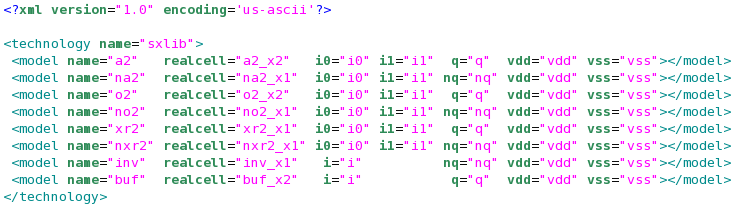
\includegraphics[width=\textwidth]{images/xml}
\end{figure}

\subsubsection{Generators}

Some generators are also provided in order to use the cells of the library with nets of more than 1 bit. One has to upper the first letter of the model name in order to user those generators. What is simply done is a for loop with the bits of the nets. The parameter \verb-'nbit'- gives the size of the generator.

\subsubsection{Example}

\begin{itemize}
    \item Direct instanciation of a cell
\end{itemize}
\begin{verbatim}
for i in range ( 4 ) :
  Inst ( 'a2'
       , map = { 'i0'  : neti0[i]
               , 'i1'  : neti1[i]
               , 'q'   : netq[i]
               , 'vdd' : netvdd
               , 'vss' : netvss
               }
       )
\end{verbatim}

\begin{itemize}
    \item Instanciation of a generator
\end{itemize}
\begin{verbatim}
Generate ( 'A2', "my_and2_4bits", param = { 'nbit' : 4 } )
Inst ( 'my_and2_4bits'
     , map  = { 'i0'  : neti0
              , 'i1'  : neti1
              , 'q'   : netq
              , 'vdd' : vdd
              , 'vss' : vss
              }
     )
\end{verbatim}

\subsubsection{Errors}
    
Some errors may occur :
\begin{itemize}
    \item \verb-[Stratus ERROR] Inst : the model ... does not exist.-\\\verb-Check CRL_CATA_LIB.-\\The model of the cell has not been found. One has to check the environment variable.
    \item \verb-[Stratus ERROR] Virtual library : No file found in order to parse.-\\\verb-Check STRATUS_MAPPING_NAME.-\\The mapping file is not given in the environment variable.
\end{itemize} 

\begin{htmlonly}
\subsubsection{See Also}

\hyperref[ref]{\emph{Introduction}}{}{Introduction}{secintroduction}

\end{htmlonly}


\begin{htmlonly}

\section{Useful links}

    \subsection{Patterns module}
    
You can find the documentation of the patterns module :\\
\url{file:///asim/coriolis/share/doc/en/html/patterns/index.html}

    \subsection{DPGEN generators}
    
You can find the documentation of the DPGEN library at :\\
\url{file:///asim/coriolis/share/doc/en/html/dpgen/index.html}

    \subsection{Arithmetic package of stratus}

You can find the documentation of the arithmetic stratus's package at :\\
\url{file:////users/outil/arith/latest/modules_stratus/arithmetic/doc/arith/index.html}

    \subsection{Arithmetic generators and some stratus packages}

You can find the documentation of the arithmetic library at :\\
\url{file:////users/outil/arith/latest/doc/index.html}

\end{htmlonly}

\end{document}
